\def\secforfig{appendices/jet-level-trigger-sf}
\def\figsversion{V1}

%\begin{figure}[ht]
%    \centering
%    \subfloat[1st jet at L1]{\label{fig:sigDiff18-1b0j-L1-1st}%
%            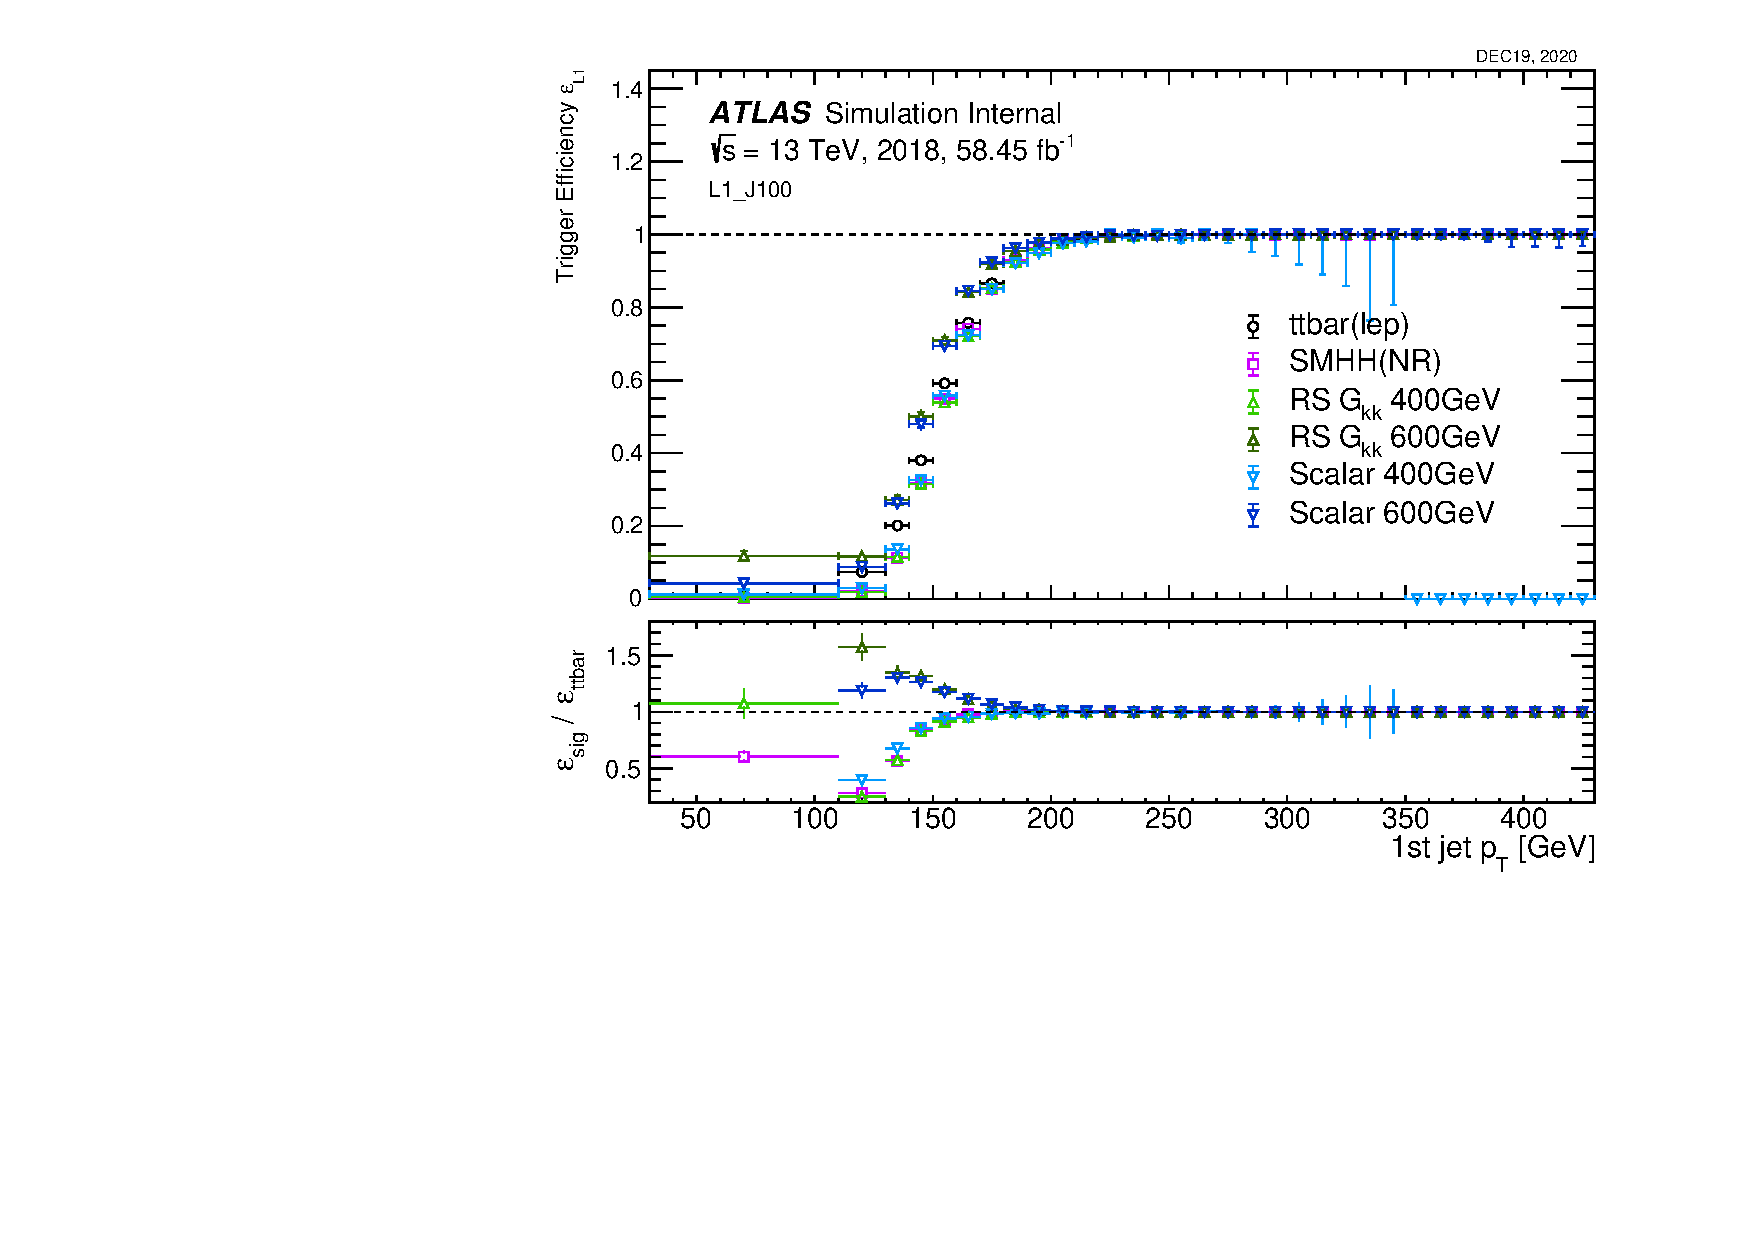
\includegraphics[width=0.25\textwidth]{\figpath{L1SDS/2018/sigDiff18-1b0j-L1-1st.pdf}}
%    }   
%
%    \subfloat[1st jet at HLT]{\label{fig:sigDiff18-1b0j-HLT-1st}%
%            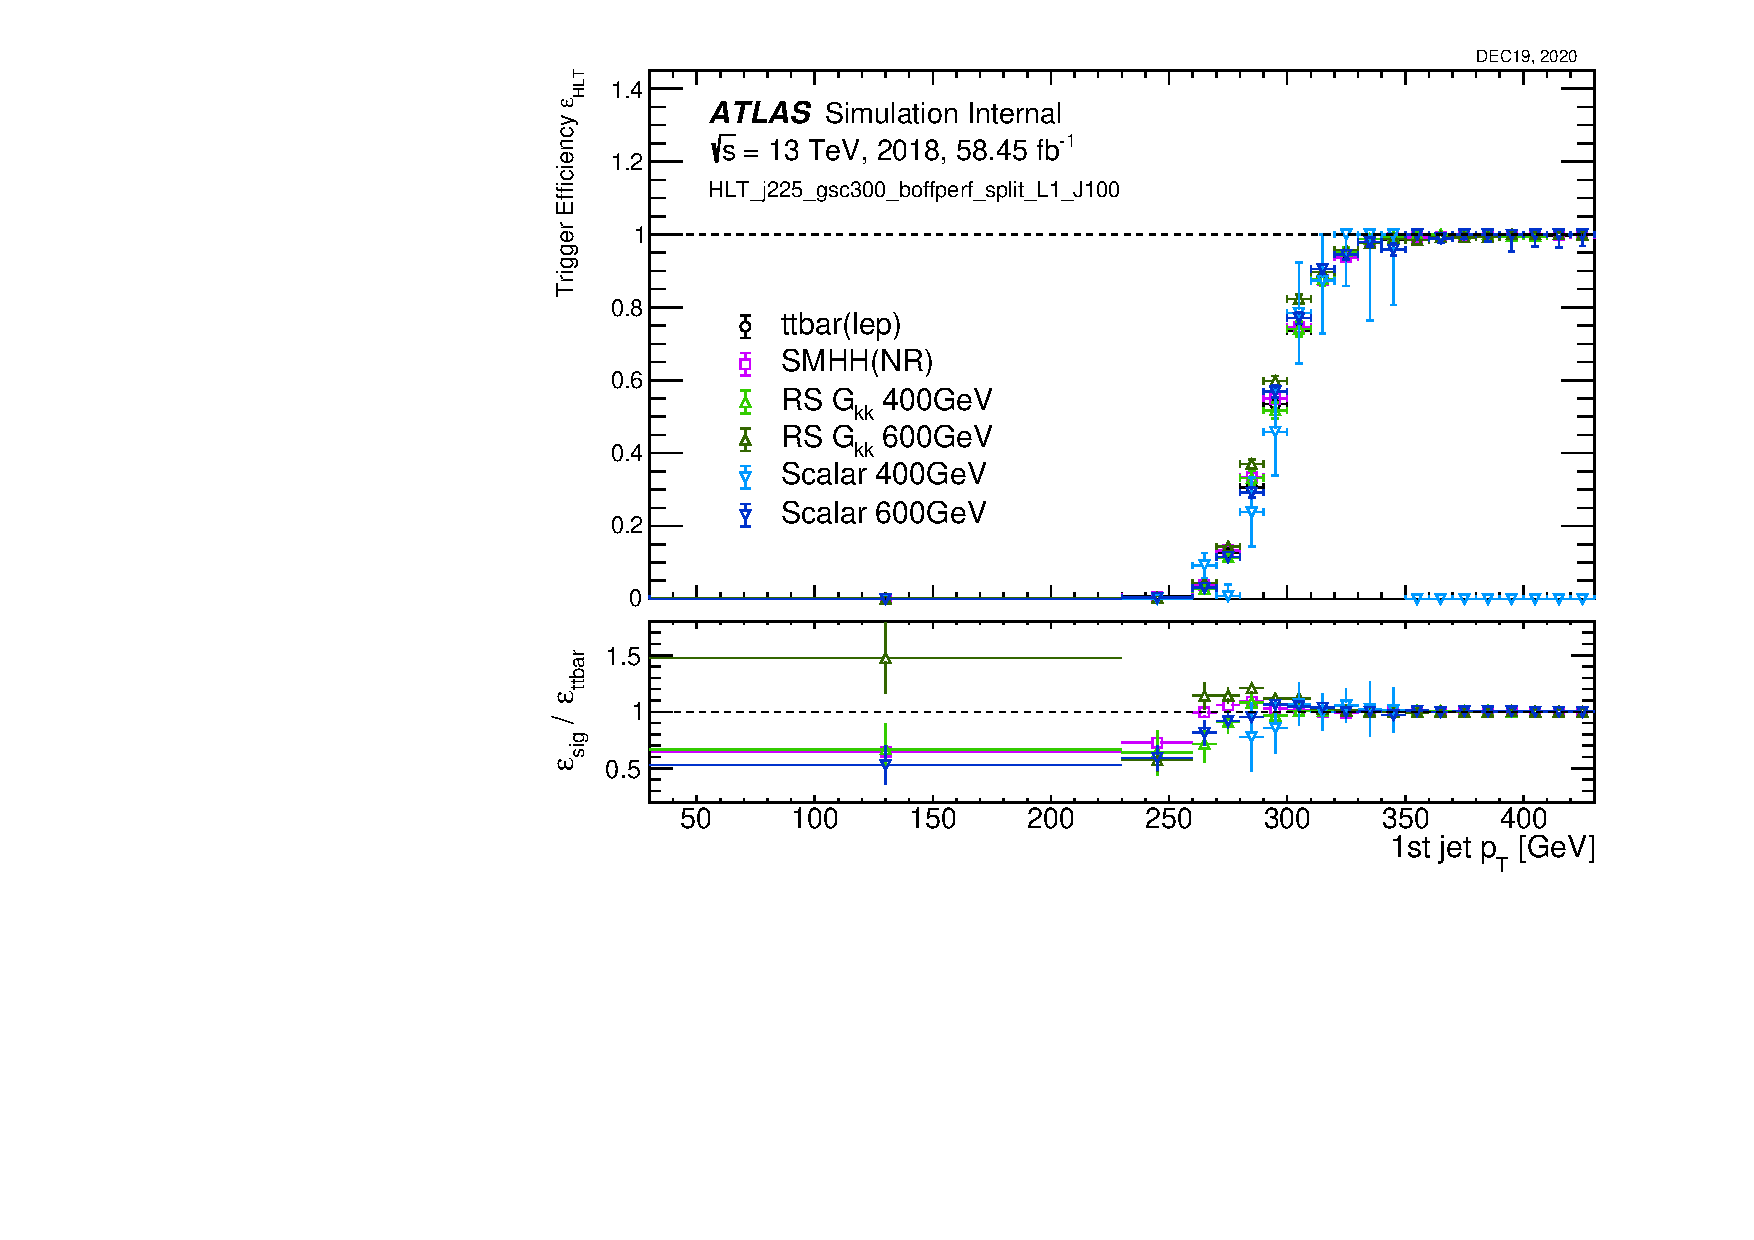
\includegraphics[width=0.25\textwidth]{\figpath{HLTSDS/2018/sigDiff18-1b0j-HLT-1st.pdf}}
%    }   
%    \caption{Jet-level trigger efficiencies of di-Higgs signals and semi-leptonic \ttbar in 2018 1b trigger as a function of offline jet \pt.
%             The Nth jet is ordered by online \et.}
%    \label{fig:sigDiff18-1b0j}
%\end{figure}
%
%\begin{figure}[ht]
%    \centering
%    \subfloat[1st jet at L1]{\label{fig:sigDiff18-2b0j-L1-1st}%
%            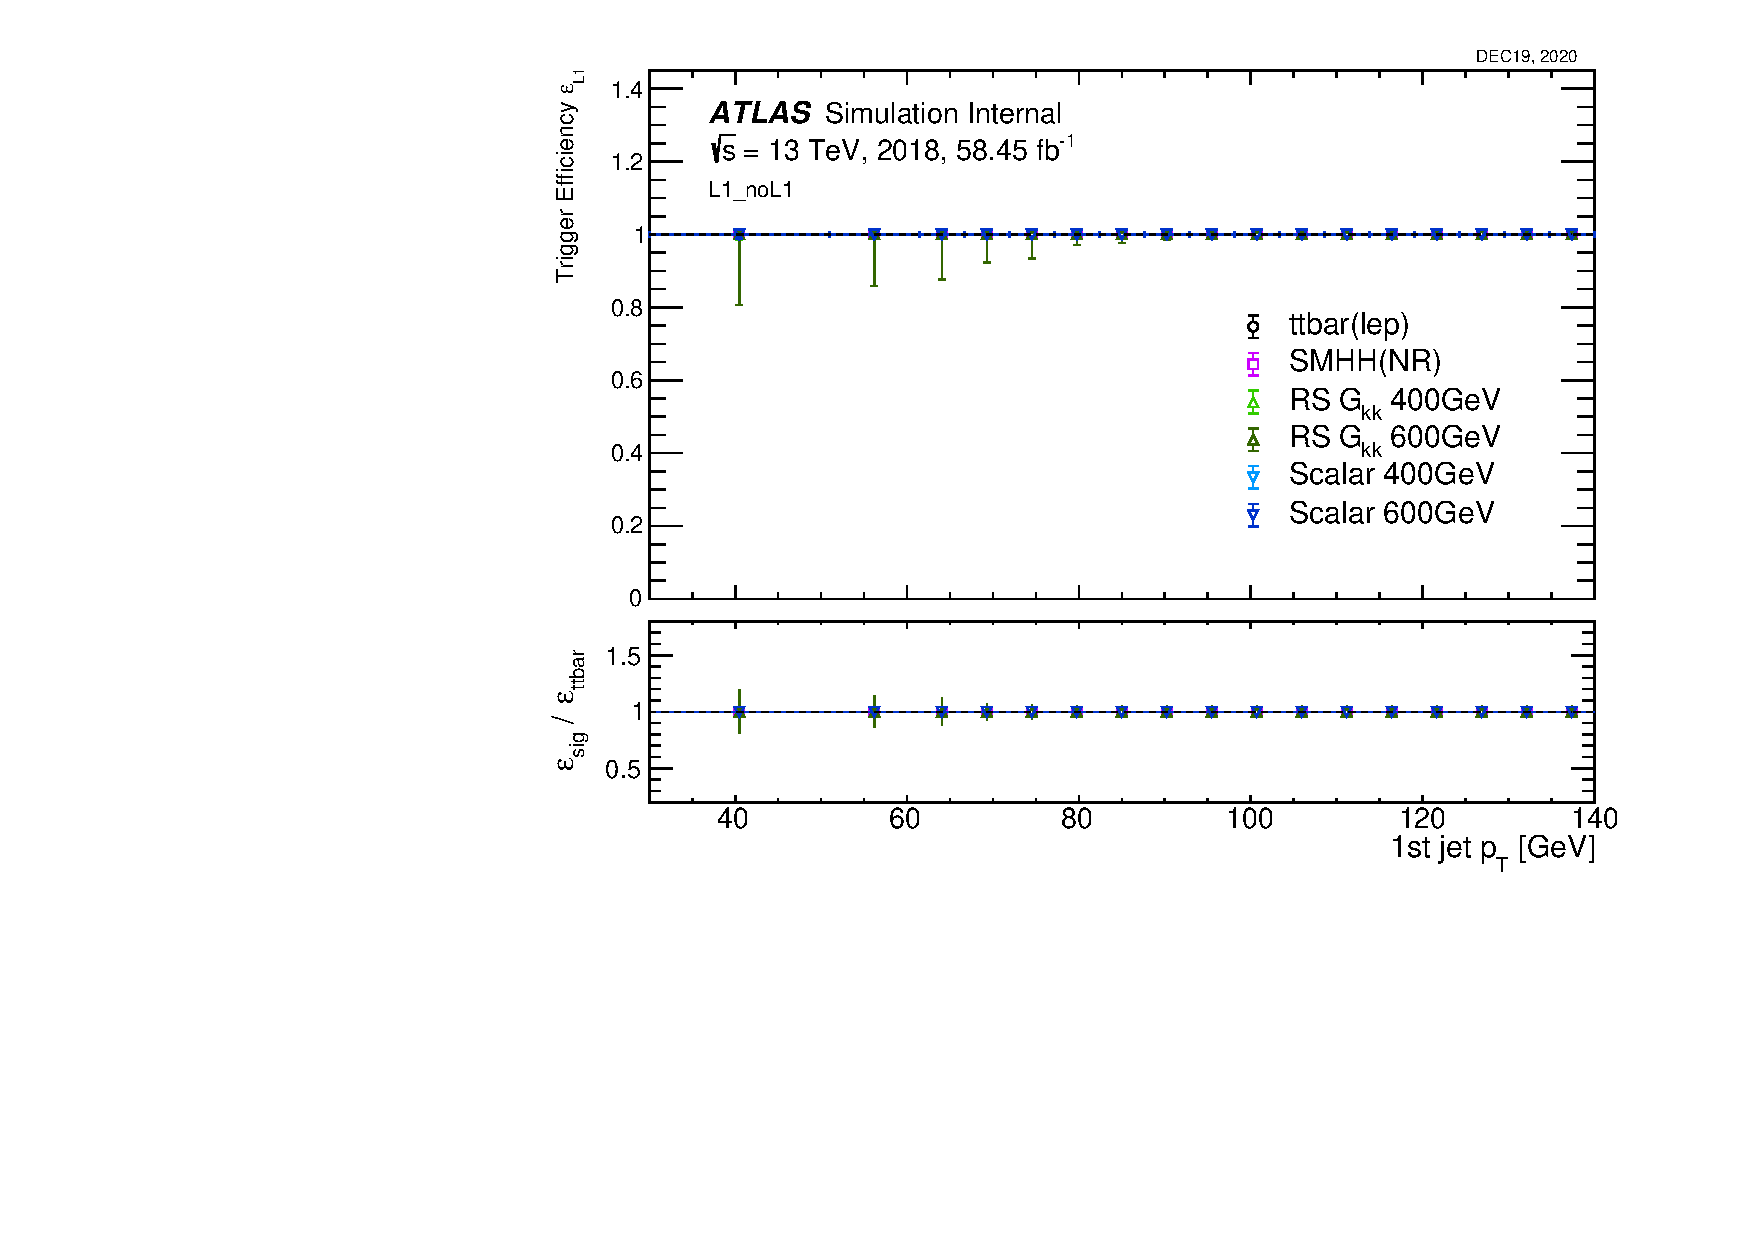
\includegraphics[width=0.25\textwidth]{\figpath{L1SDS/2018/sigDiff18-2b0j-L1-1st.pdf}}
%    }   
%    \subfloat[2nd jet at L1]{\label{fig:sigDiff18-2b0j-L1-2nd}%
%            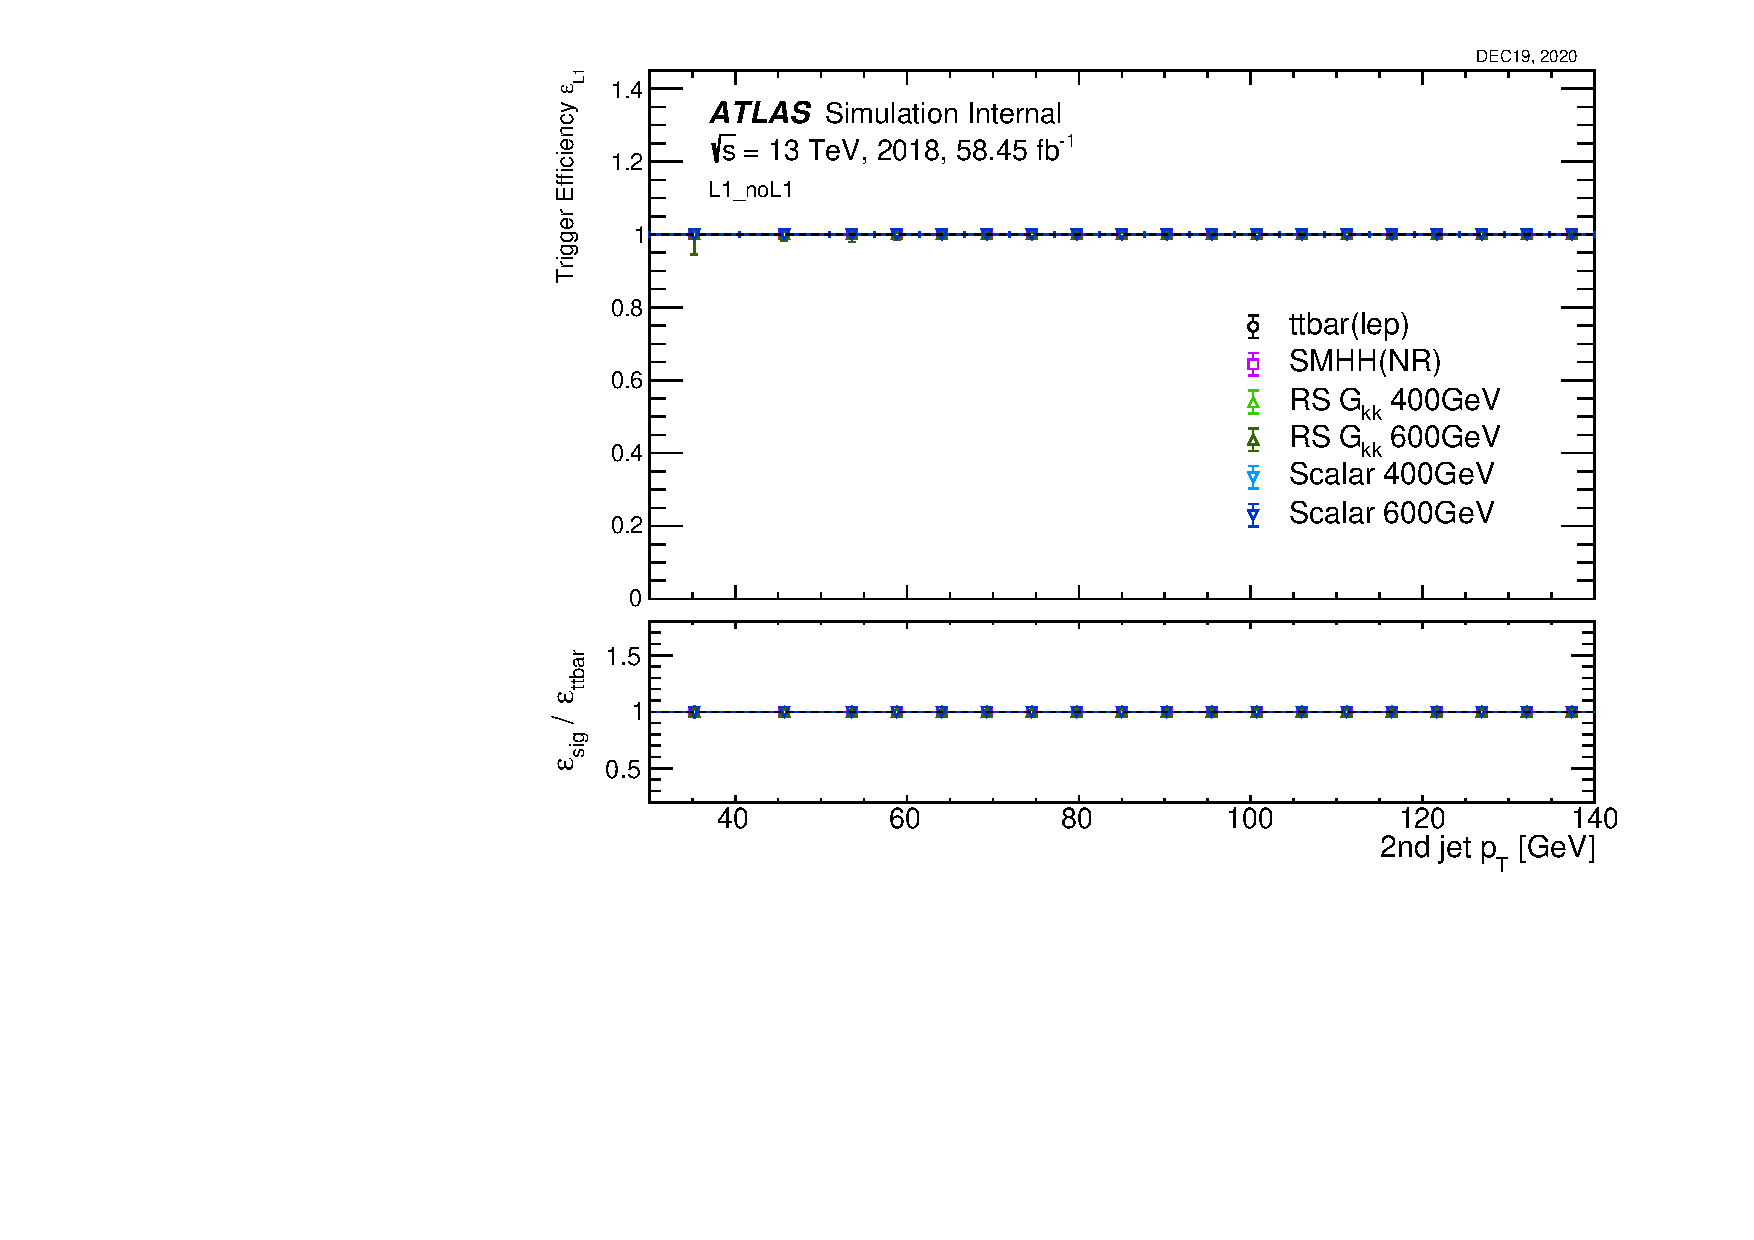
\includegraphics[width=0.25\textwidth]{\figpath{L1SDS/2018/sigDiff18-2b0j-L1-2nd.pdf}}
%    }   
%    \subfloat[HT jet at L1]{\label{fig:sigDiff18-2b0j-L1-HT}%
%            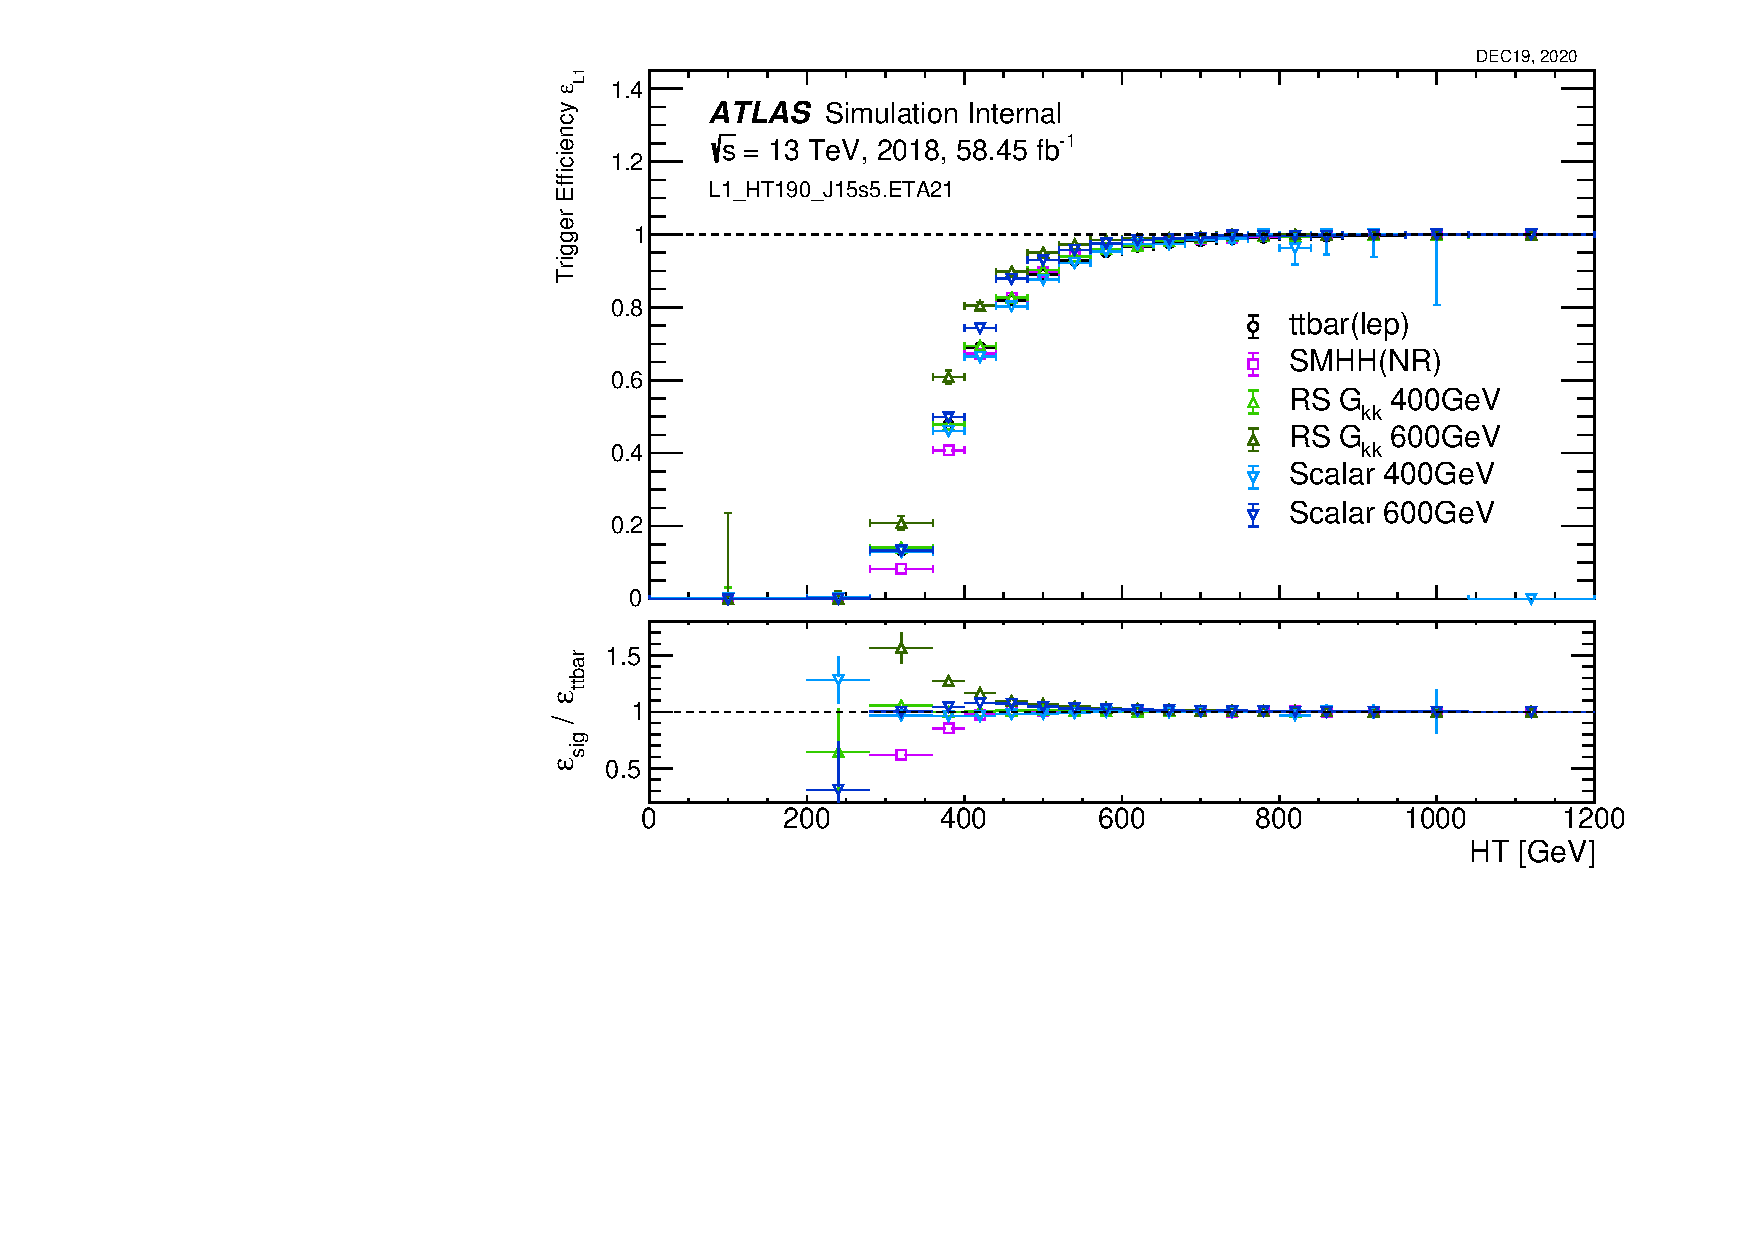
\includegraphics[width=0.25\textwidth]{\figpath{L1SDS/2018/sigDiff18-2b0j-L1-HT.pdf}}
%    }   
% 
%    \subfloat[1st jet at HLT]{\label{fig:sigDiff18-2b0j-HLT-1st}%
%            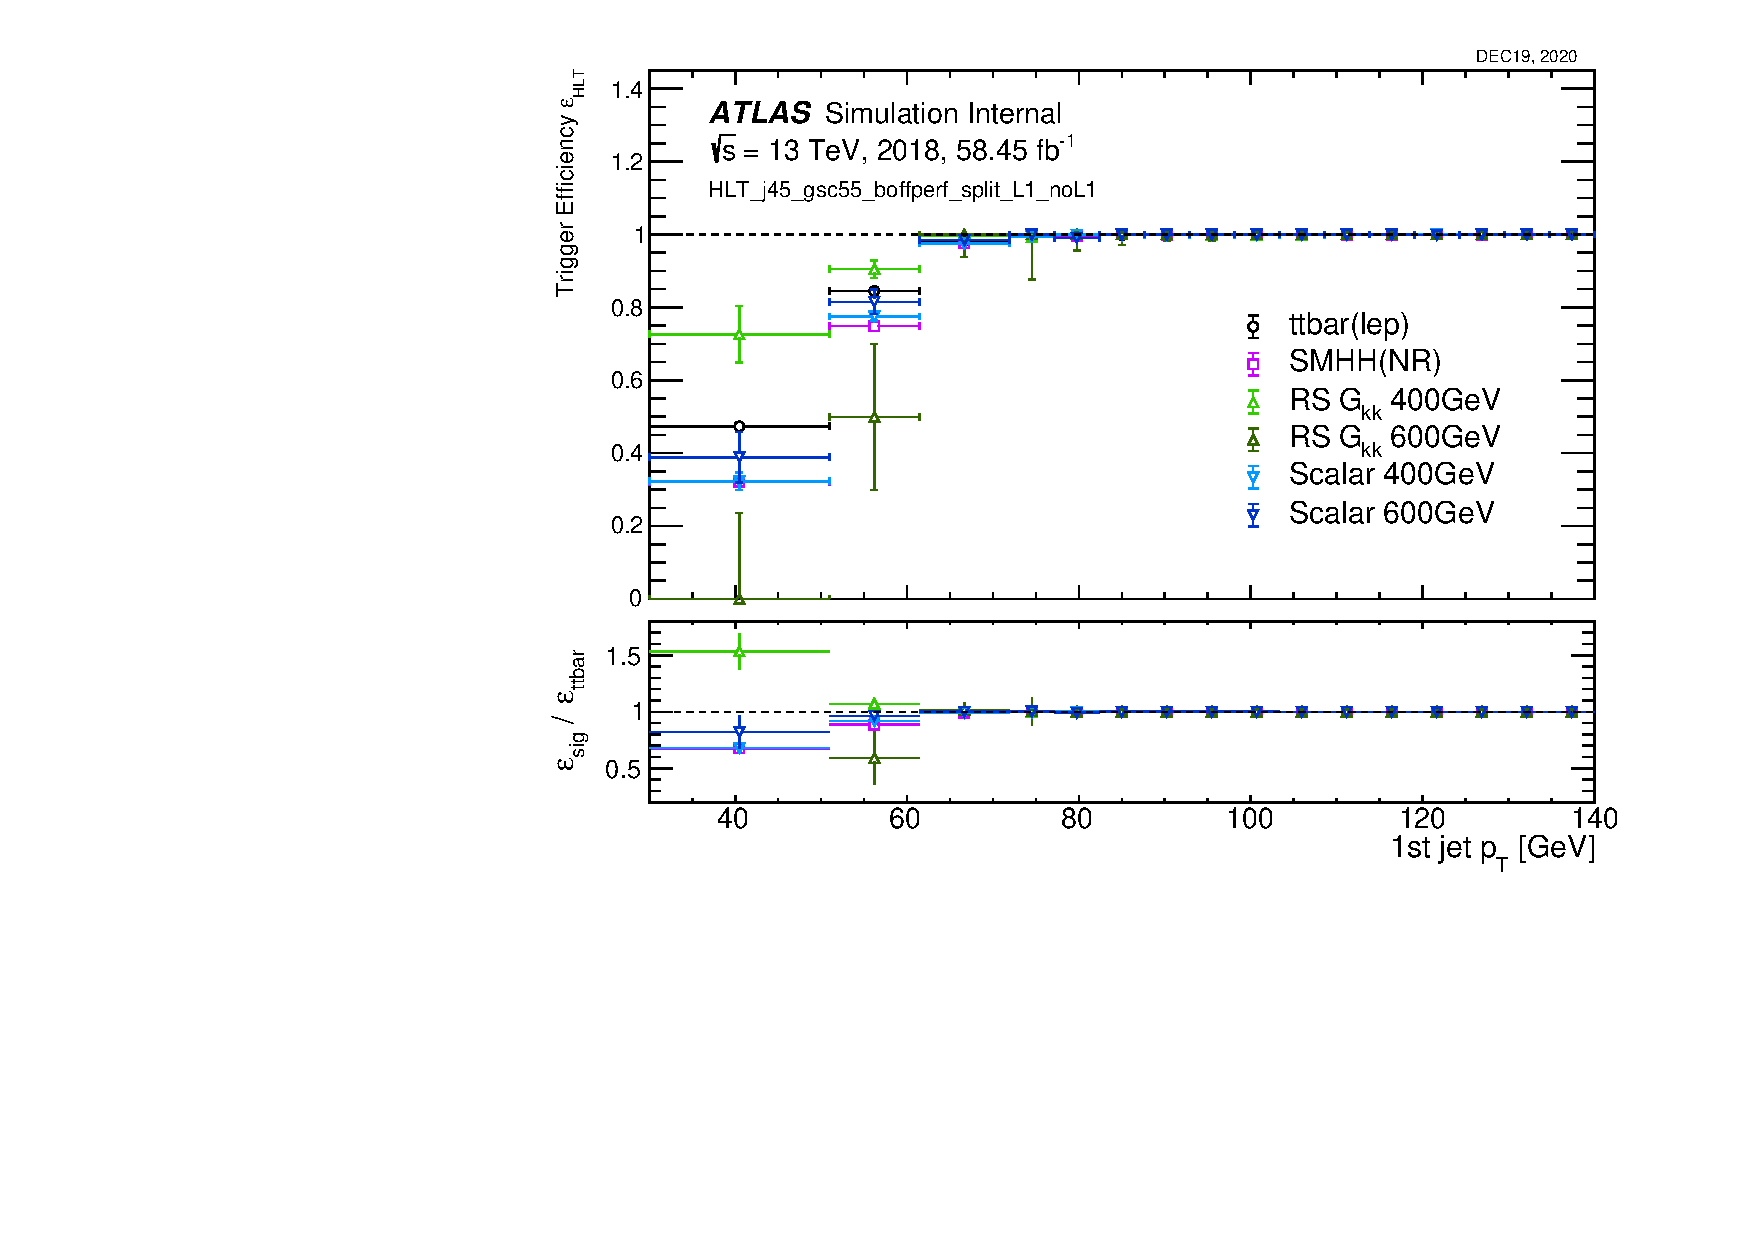
\includegraphics[width=0.25\textwidth]{\figpath{HLTSDS/2018/sigDiff18-2b0j-HLT-1st.pdf}}
%    }   
%    \subfloat[2nd jet at HLT]{\label{fig:sigDiff18-2b0j-HLT-2nd}%
%            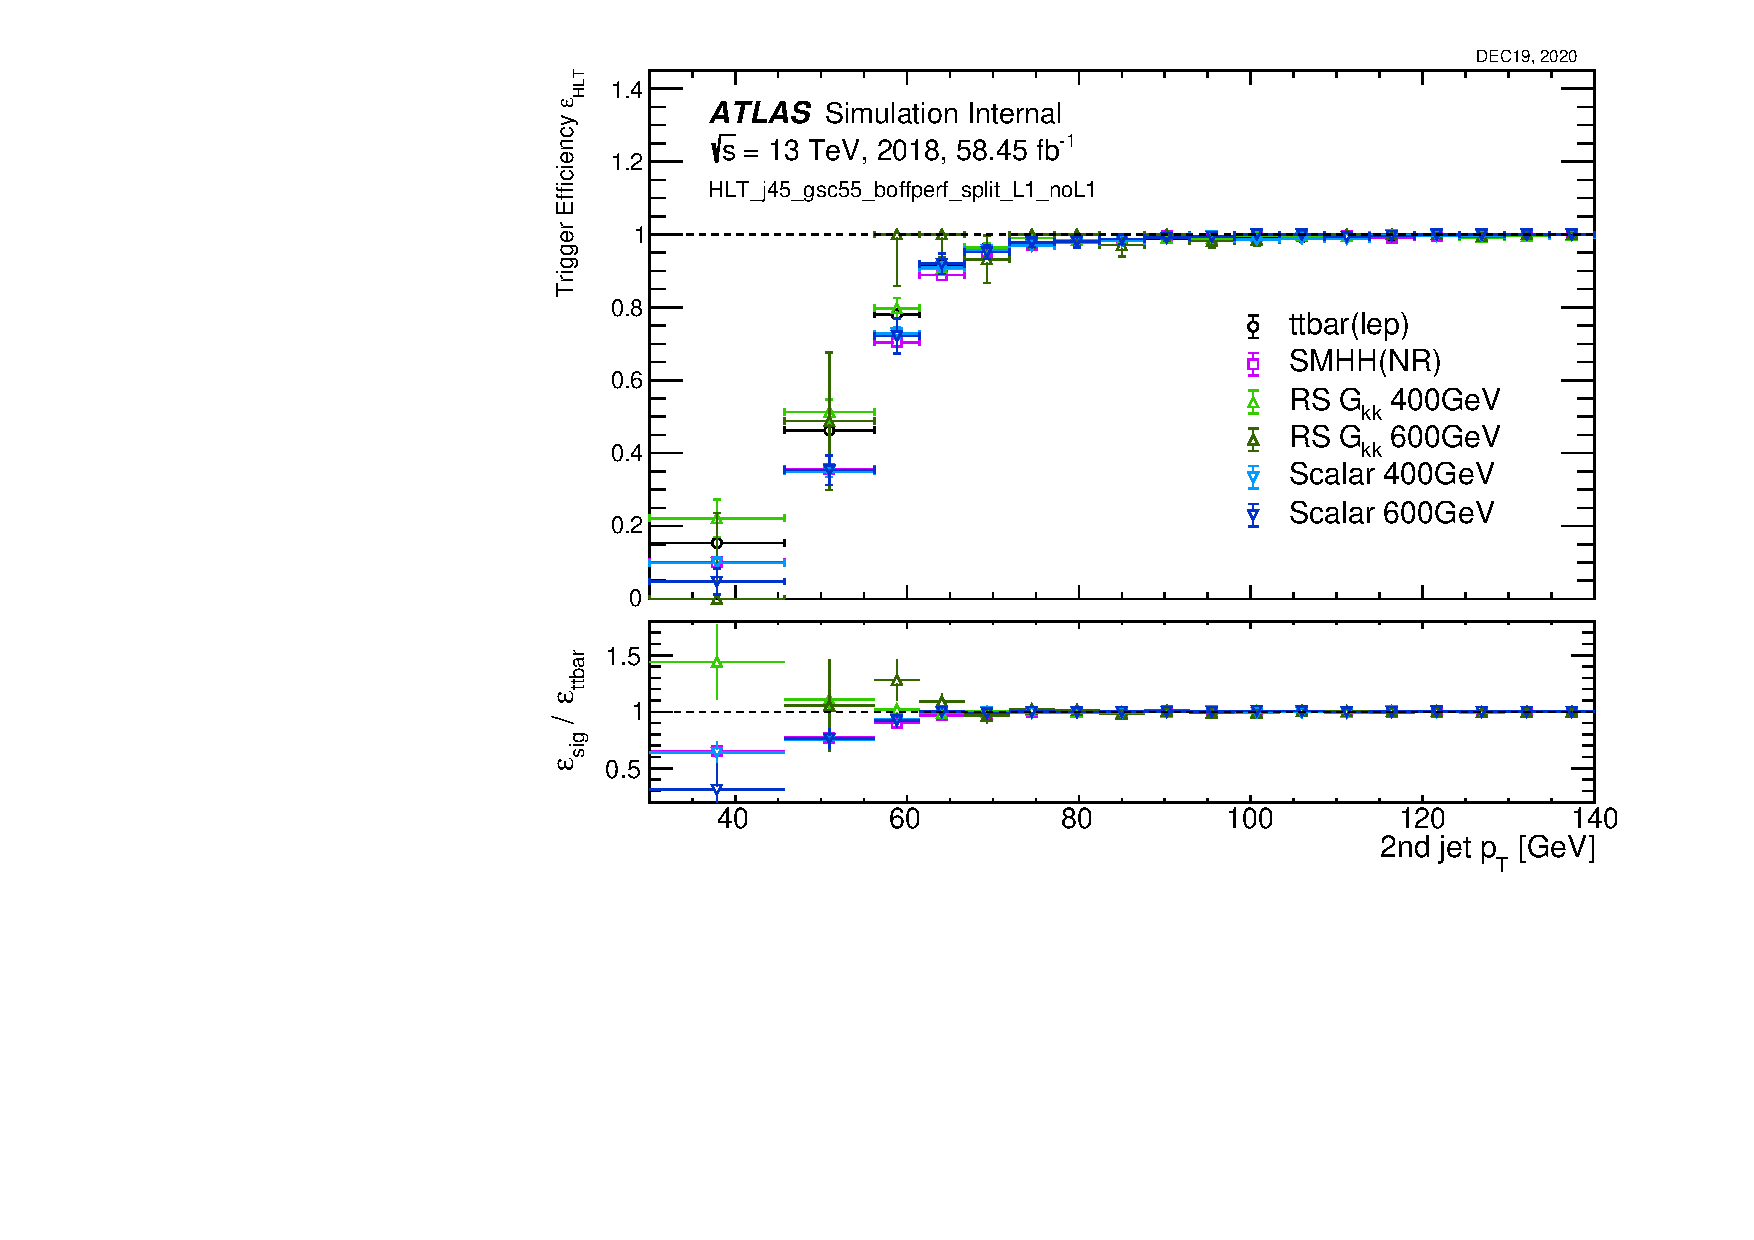
\includegraphics[width=0.25\textwidth]{\figpath{HLTSDS/2018/sigDiff18-2b0j-HLT-2nd.pdf}}
%    }   
%    \subfloat[HT jet at HLT]{\label{fig:sigDiff18-2b0j-HLT-HT}%
%            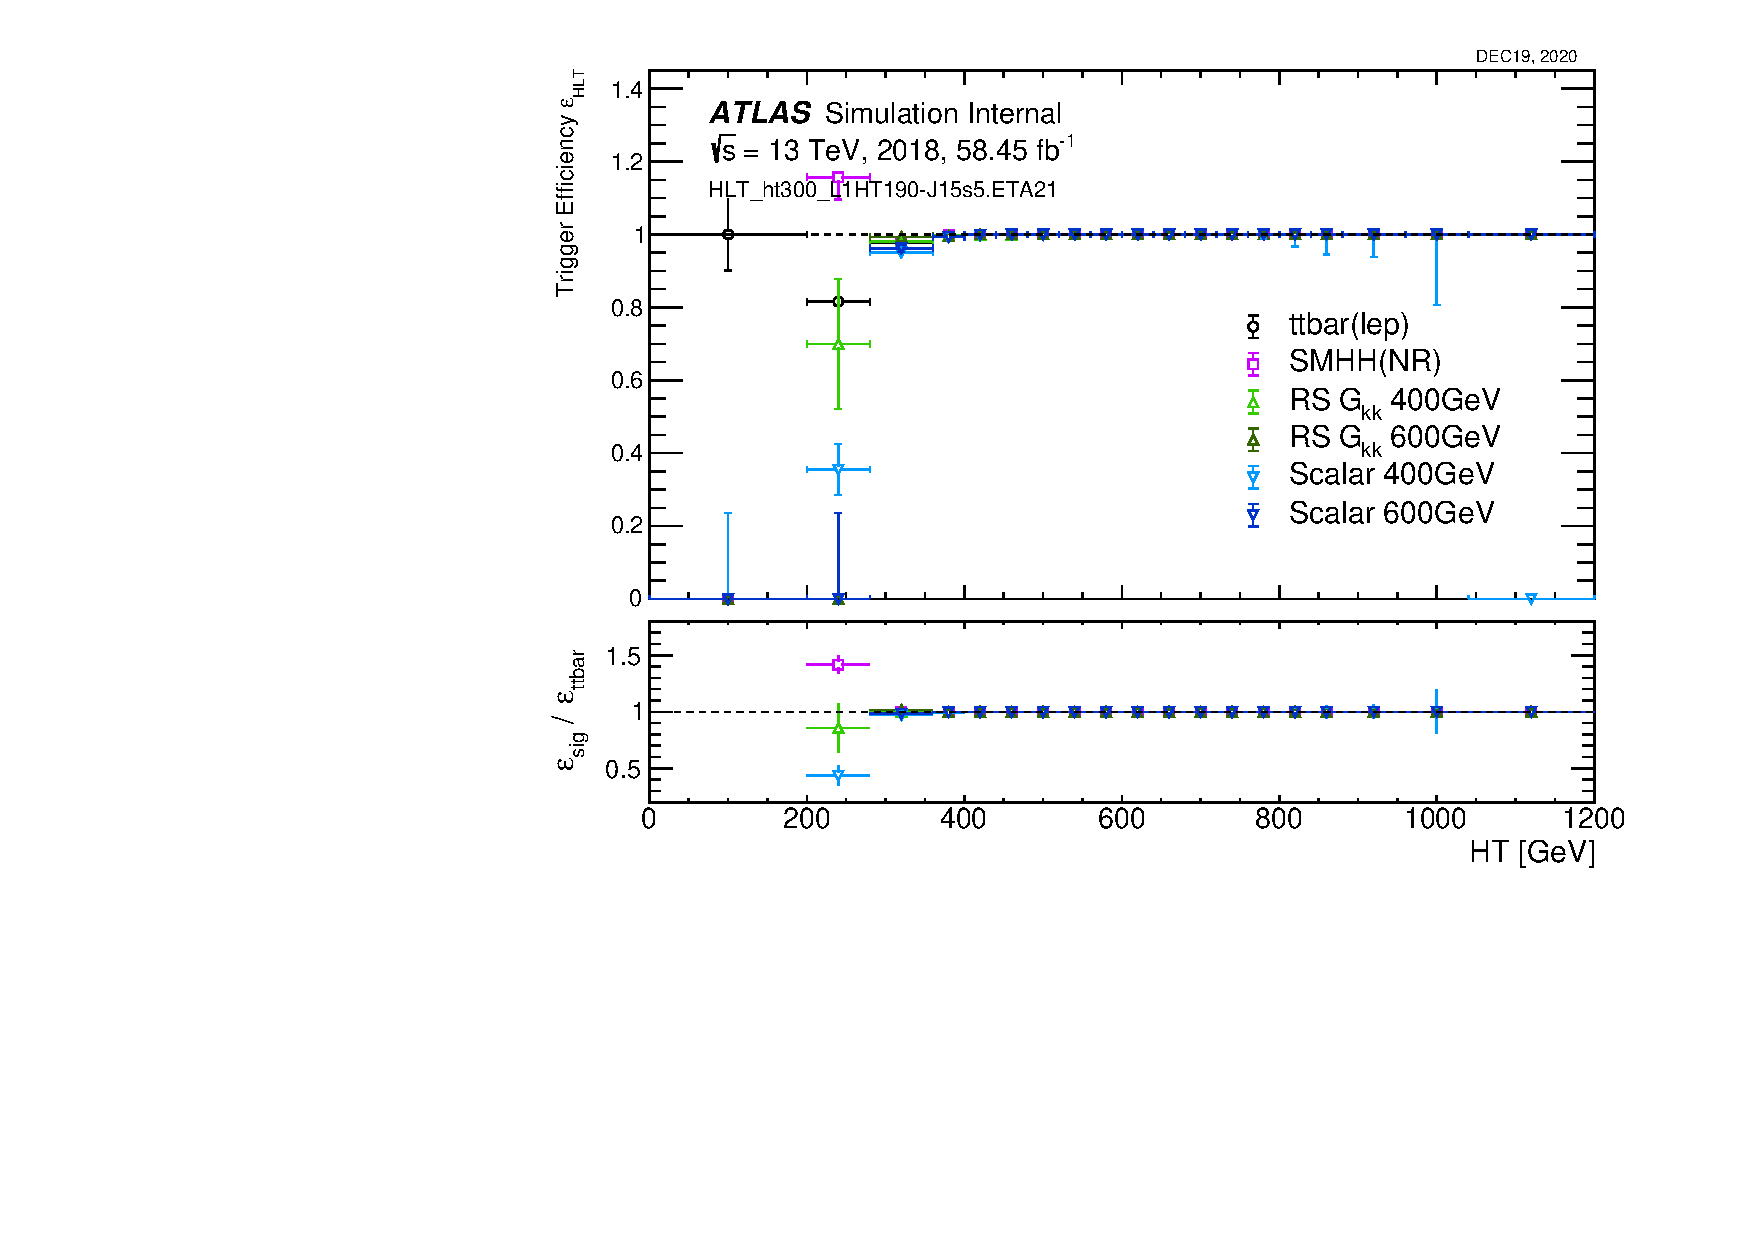
\includegraphics[width=0.25\textwidth]{\figpath{HLTSDS/2018/sigDiff18-2b0j-HLT-HT.pdf}}
%    }   
%    \caption{Jet-level trigger efficiencies of di-Higgs signals and semi-leptonic \ttbar in 2018 2bHT trigger as a function of offline jet \pt.
%             The Nth jet is ordered by online \et.}
%    \label{fig:sigDiff18-2bHT}
%\end{figure}

\begin{figure}[ht]
    \centering
    \subfloat[1st jet at L1]{\label{fig:sigDiff18-2b1j-L1-1st}%
            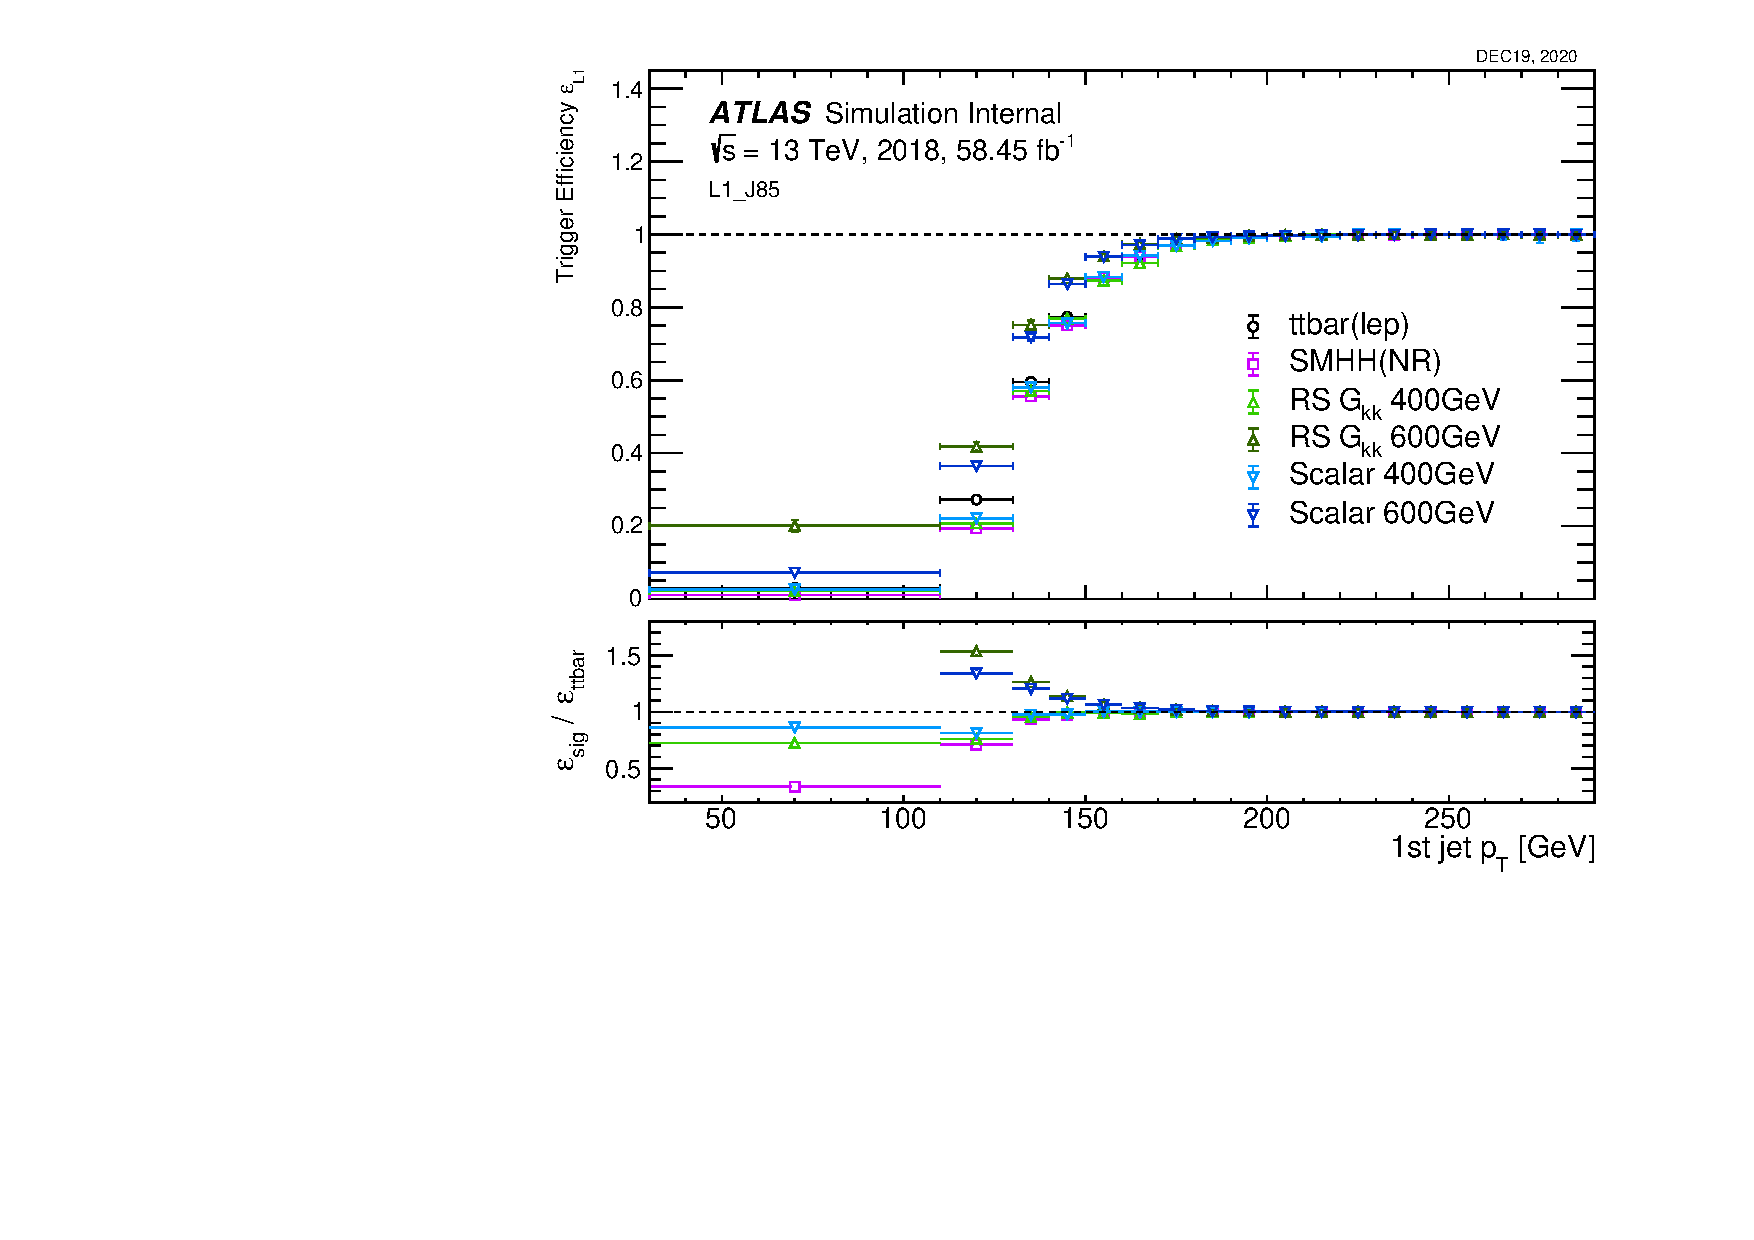
\includegraphics[width=0.25\textwidth]{\figpath{L1SDS/2018/sigDiff18-2b1j-L1-1st.pdf}}
    }   
    \subfloat[2nd jet at L1]{\label{fig:sigDiff18-2b1j-L1-2nd}%
            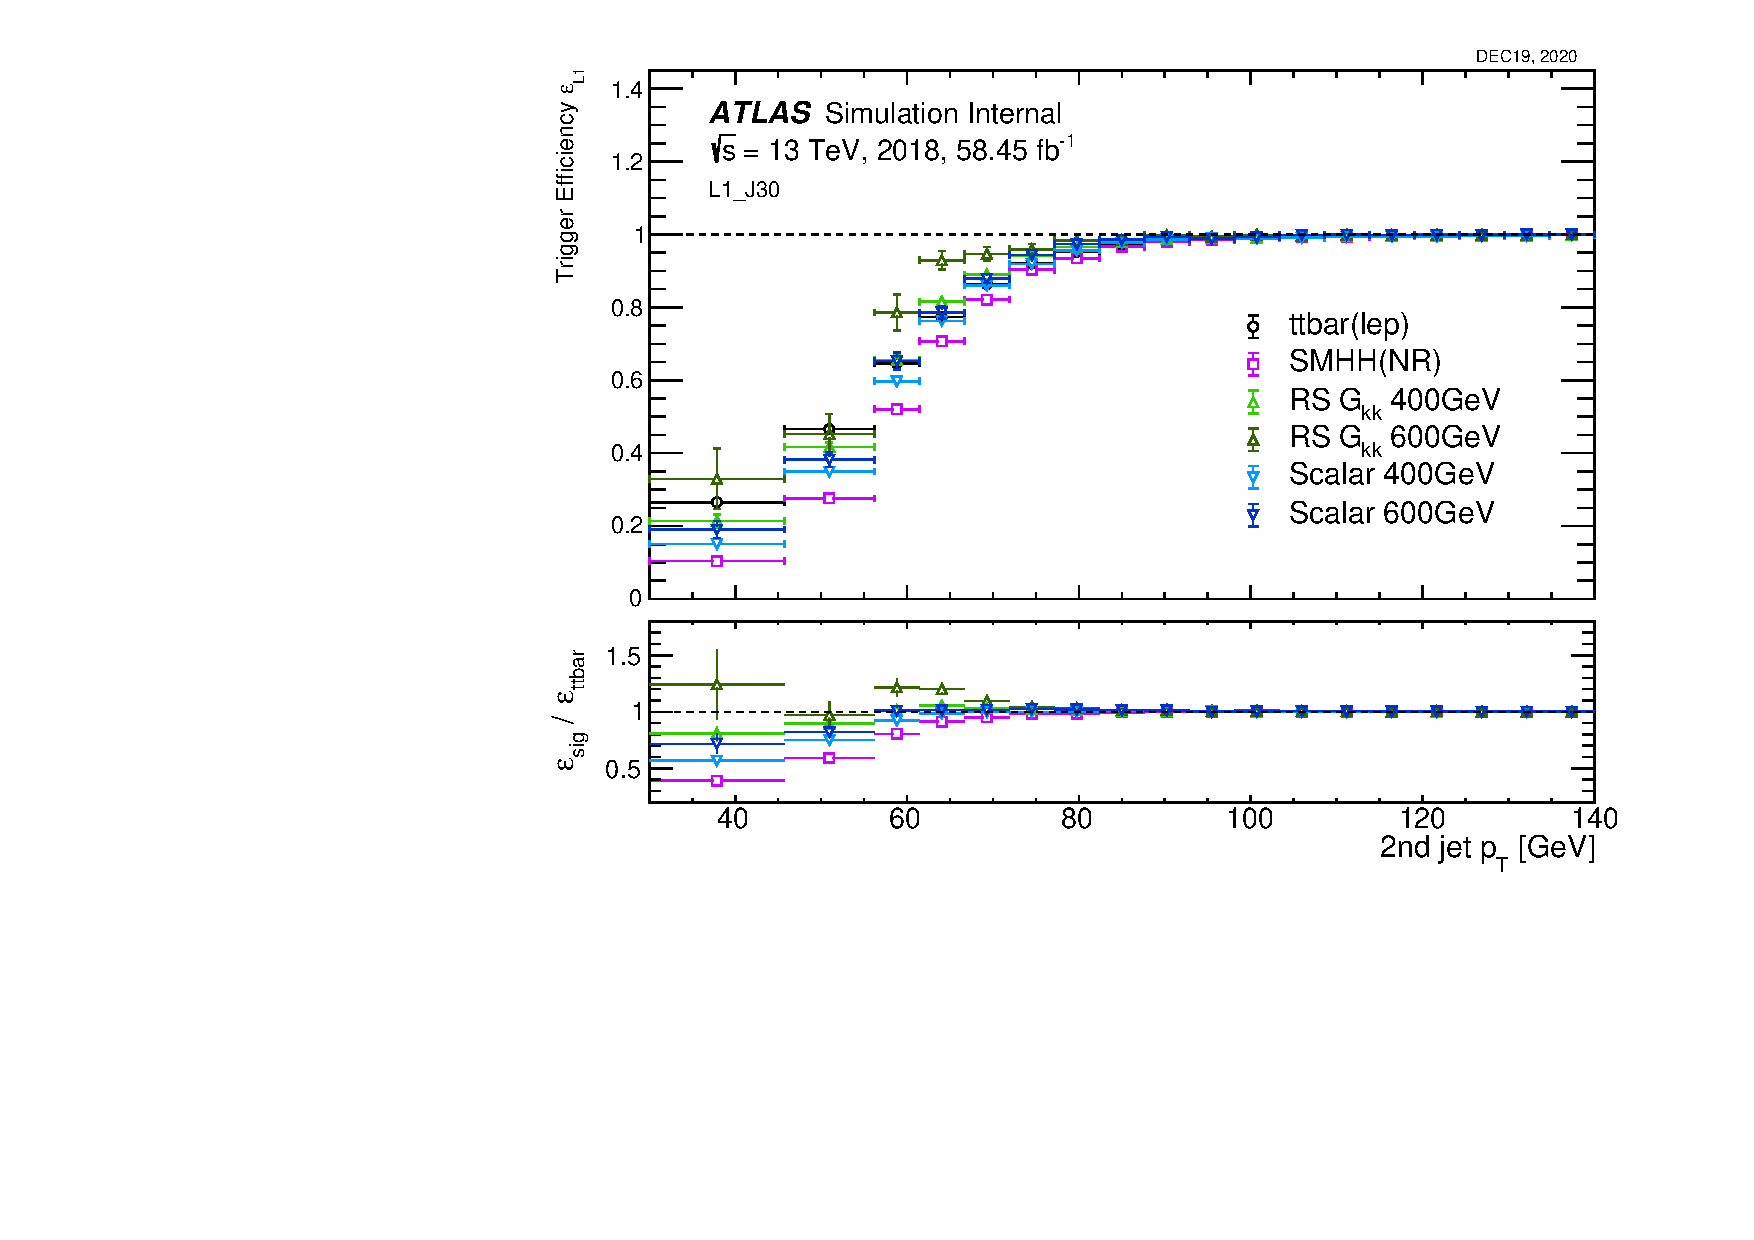
\includegraphics[width=0.25\textwidth]{\figpath{L1SDS/2018/sigDiff18-2b1j-L1-2nd.pdf}}
    }   
    \subfloat[3rd jet at L1]{\label{fig:sigDiff18-2b1j-L1-3rd}%
            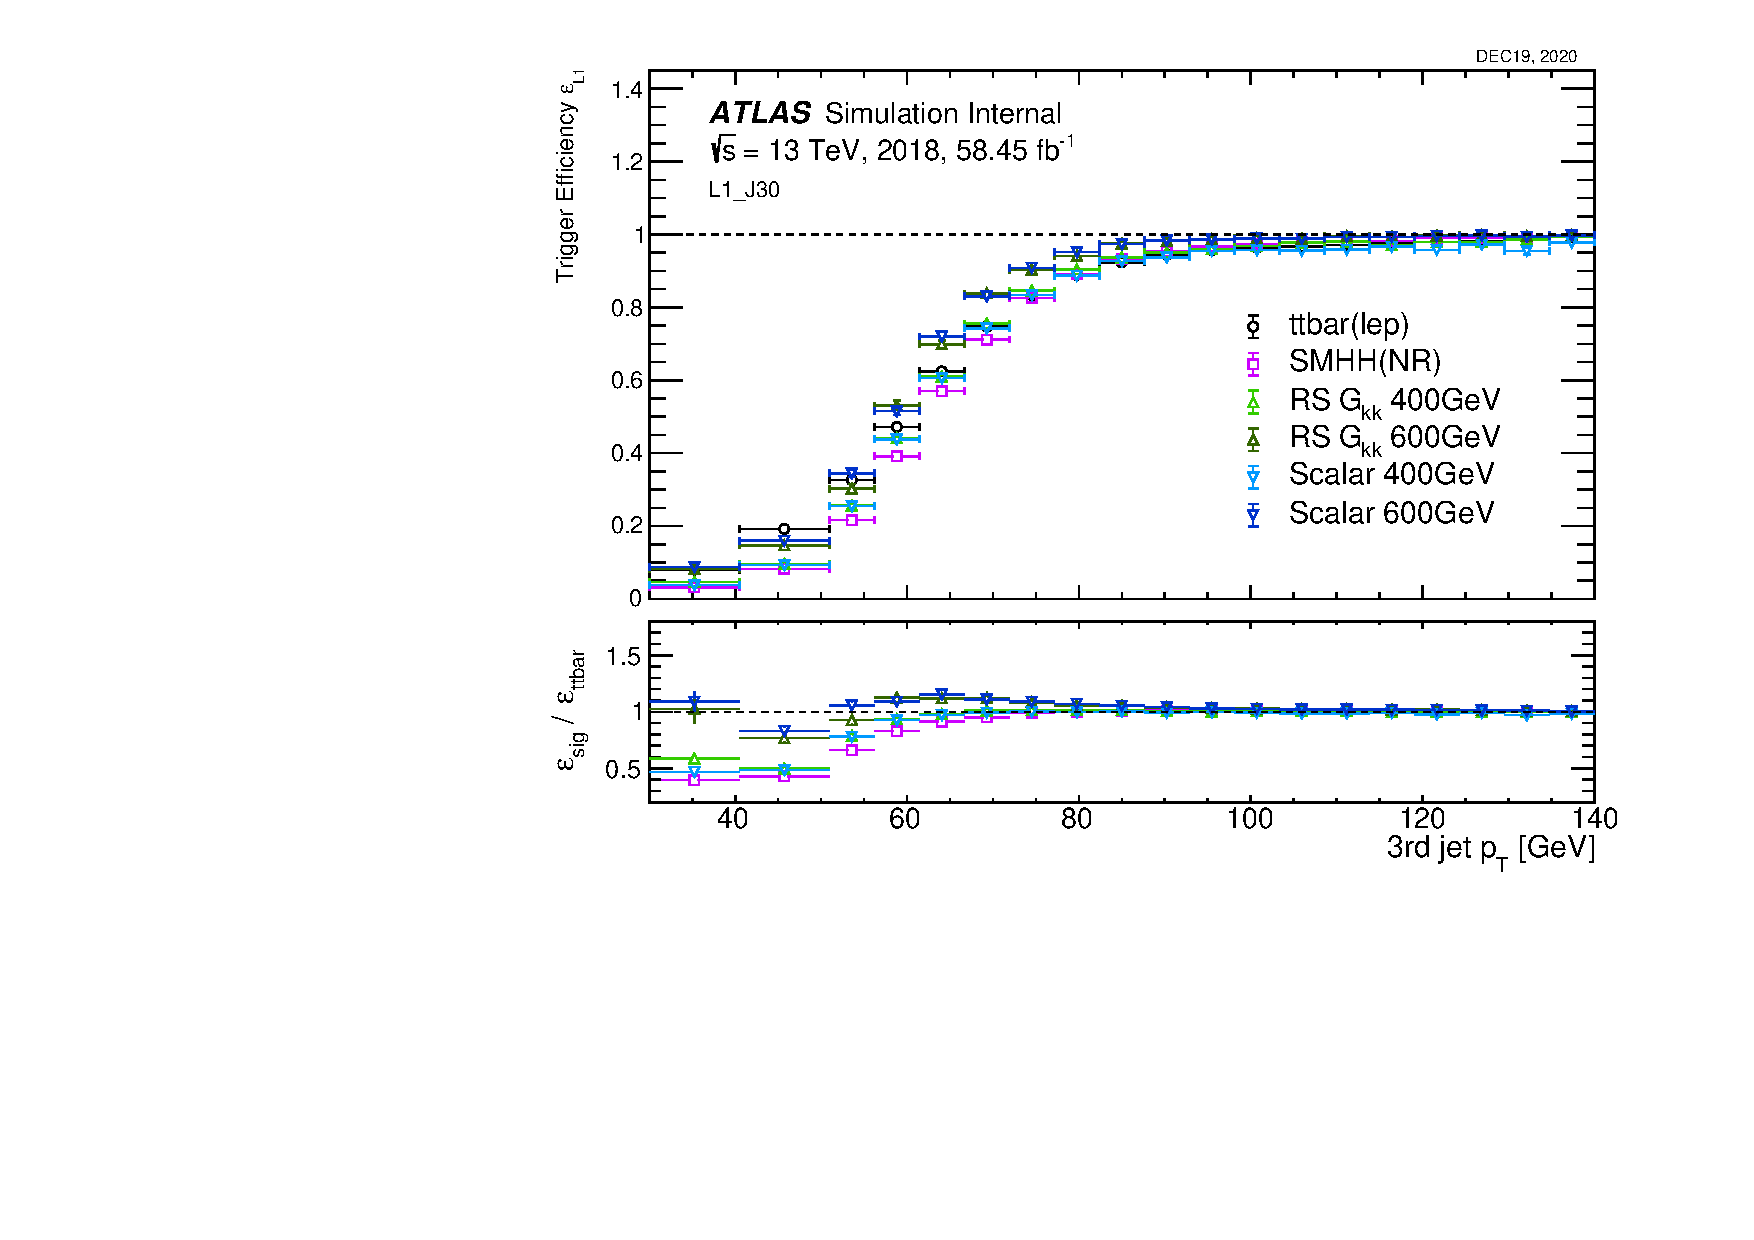
\includegraphics[width=0.25\textwidth]{\figpath{L1SDS/2018/sigDiff18-2b1j-L1-3rd.pdf}}
    }   
 
    \subfloat[1st jet at HLT]{\label{fig:sigDiff18-2b1j-HLT-1st}%
            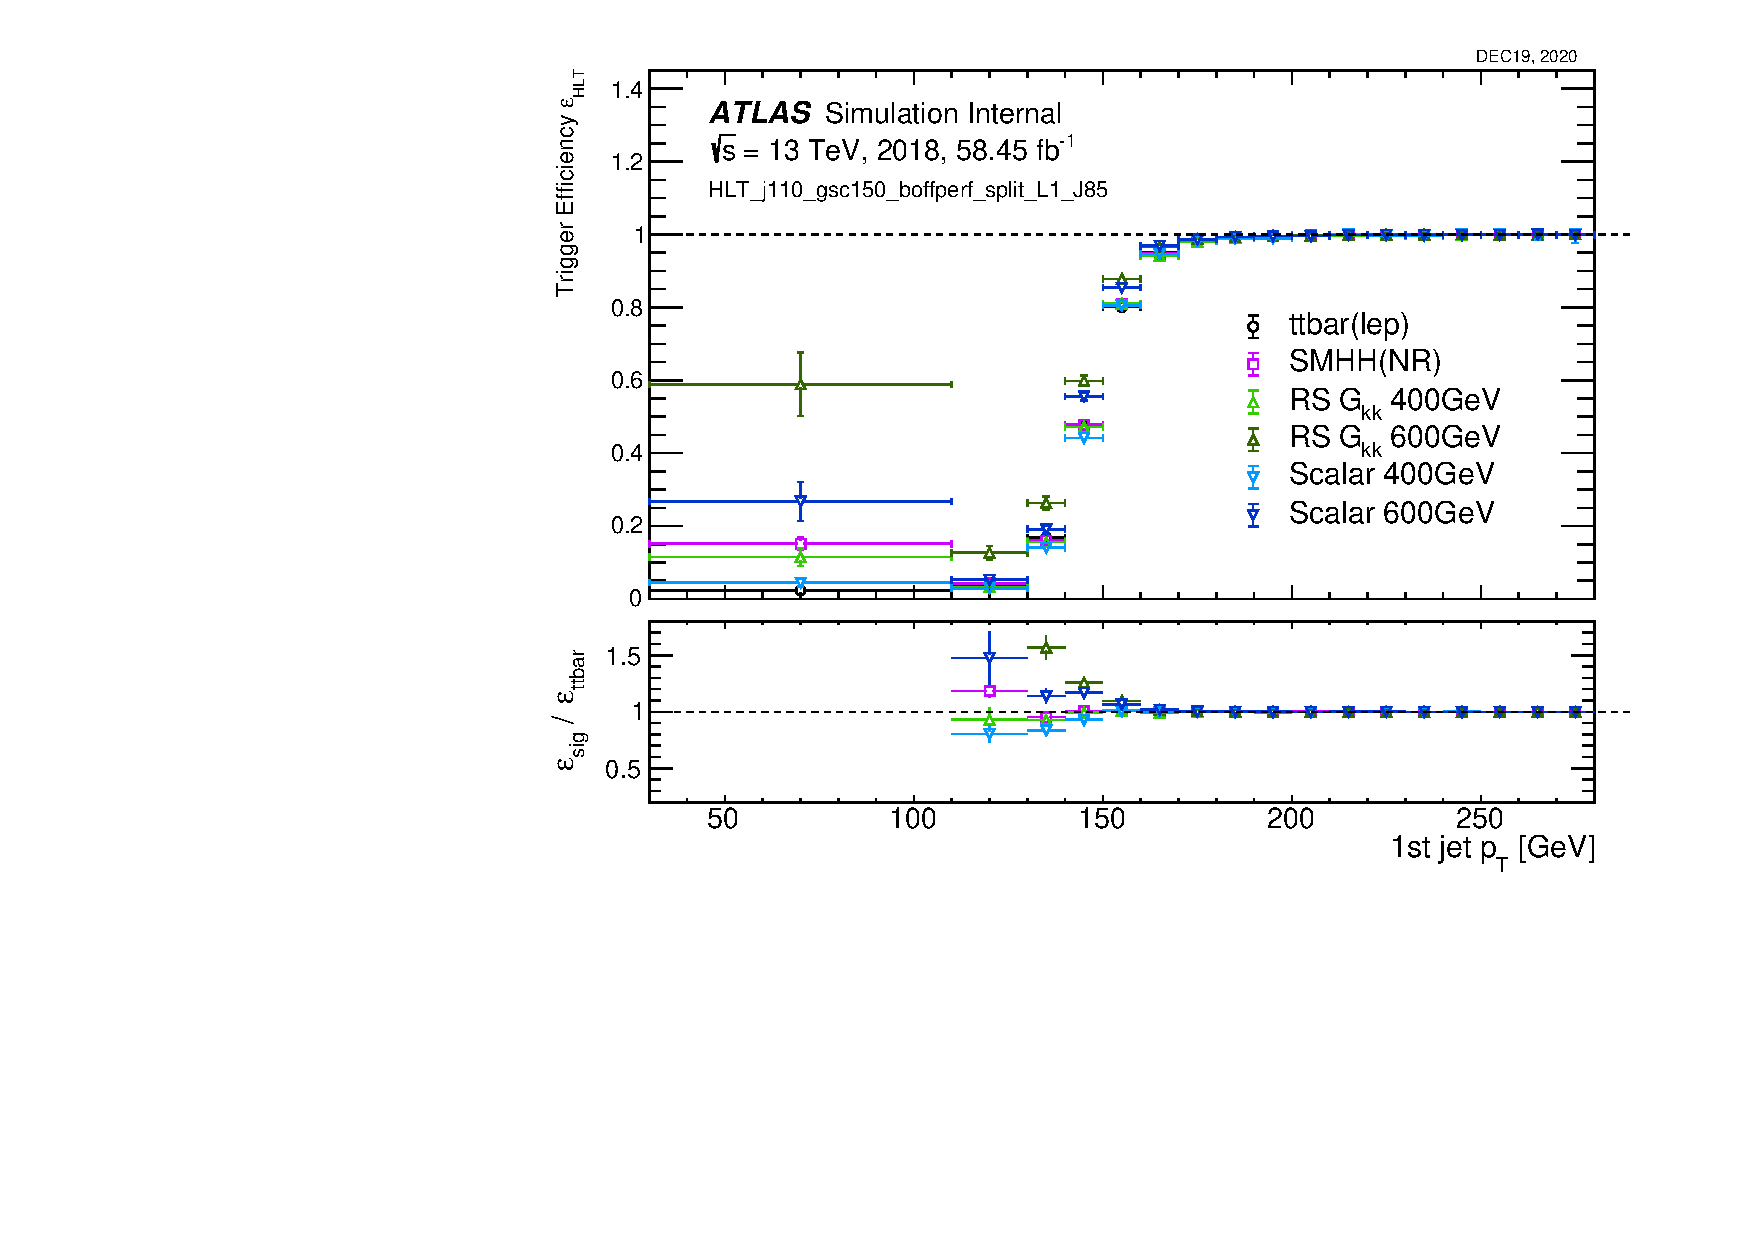
\includegraphics[width=0.25\textwidth]{\figpath{HLTSDS/2018/sigDiff18-2b1j-HLT-1st.pdf}}
    }   
    \subfloat[2nd jet at HLT]{\label{fig:sigDiff18-2b1j-HLT-2nd}%
            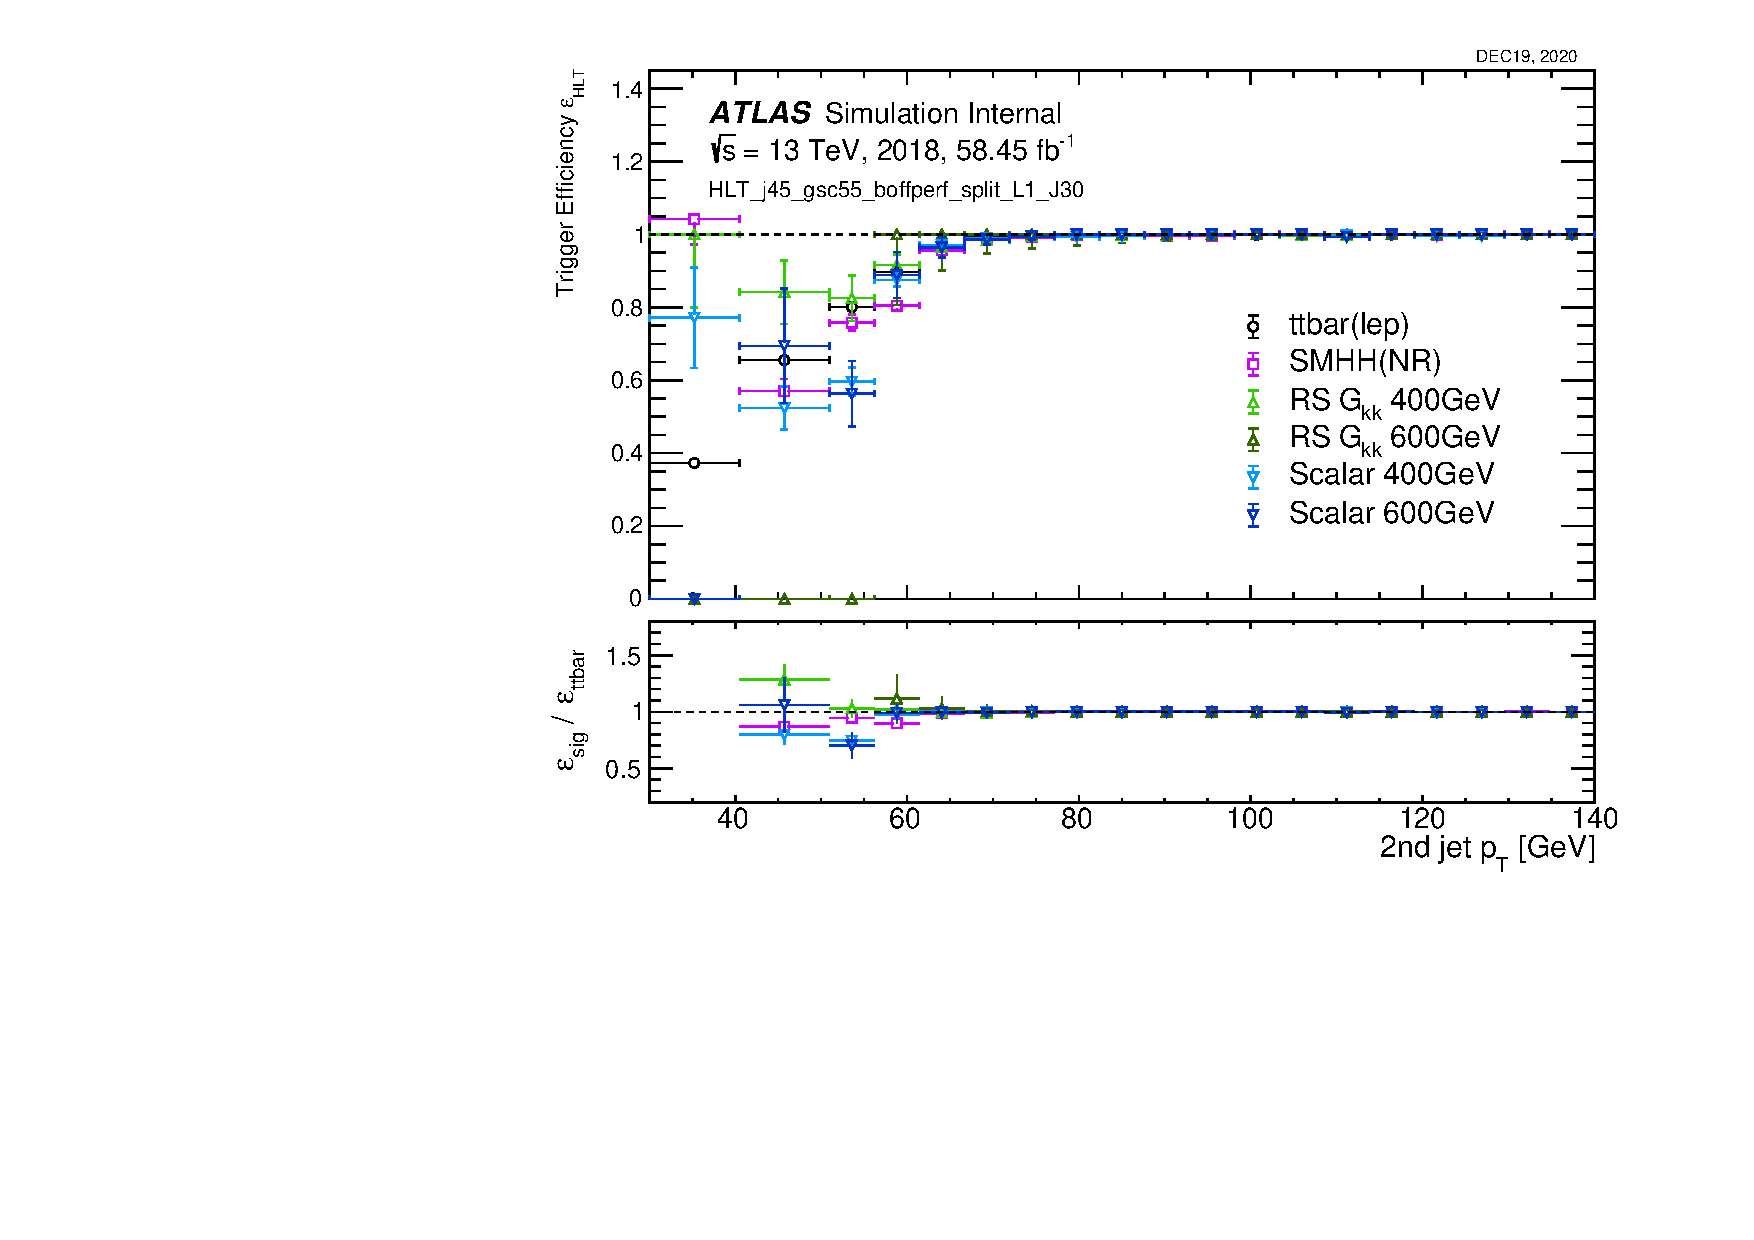
\includegraphics[width=0.25\textwidth]{\figpath{HLTSDS/2018/sigDiff18-2b1j-HLT-2nd.pdf}}
    }   
    \subfloat[3rd jet at HLT]{\label{fig:sigDiff18-2b1j-HLT-3rd}%
            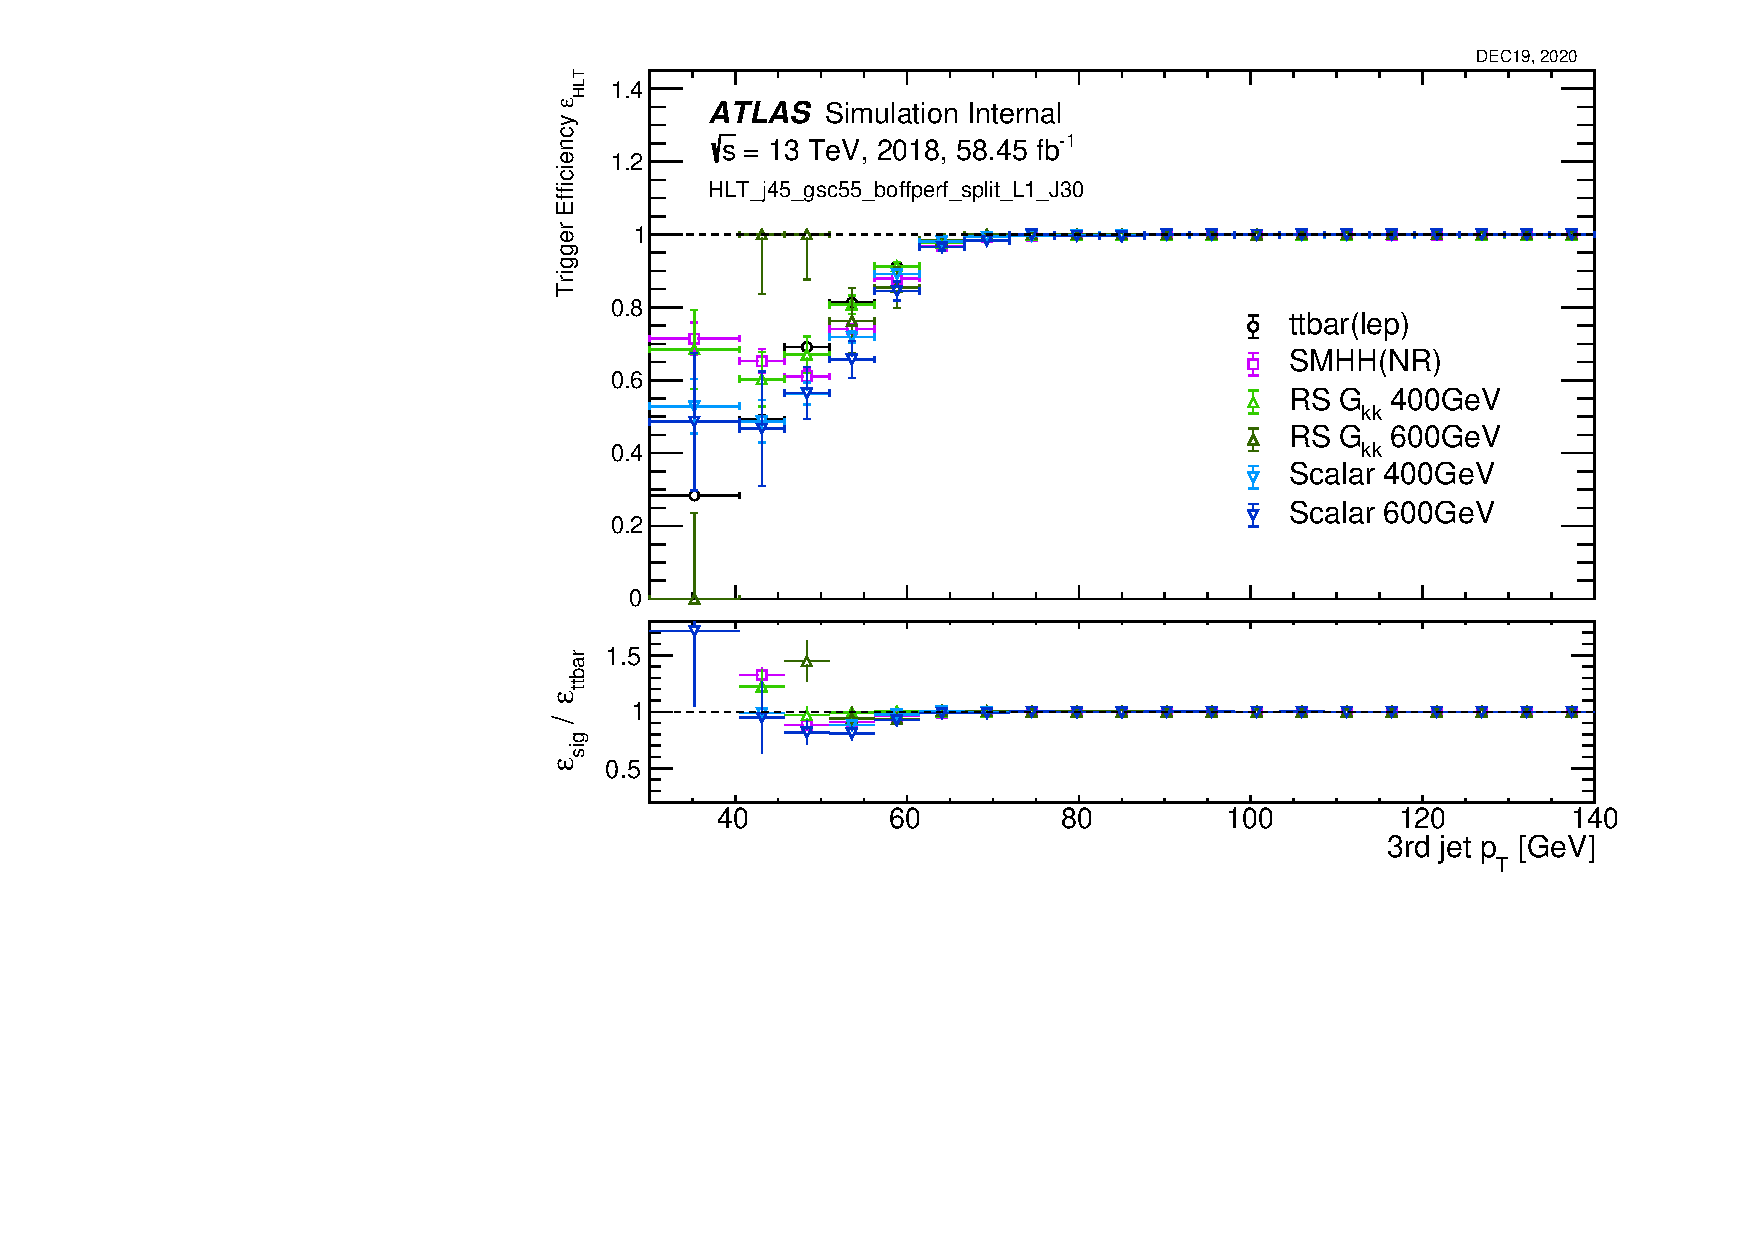
\includegraphics[width=0.25\textwidth]{\figpath{HLTSDS/2018/sigDiff18-2b1j-HLT-3rd.pdf}}
    }   
    \caption{Jet-level trigger efficiencies of di-Higgs signals and semi-leptonic \ttbar in 2018 2b1j trigger as a function of offline jet \pt.
             The Nth jet is ordered by online \et.}
    \label{fig:sigDiff18-2b1j}
\end{figure}

\begin{figure}[ht]
    \centering
    \subfloat[1st jet at L1]{\label{fig:sigDiff18-2b2j-L1-1st}%
            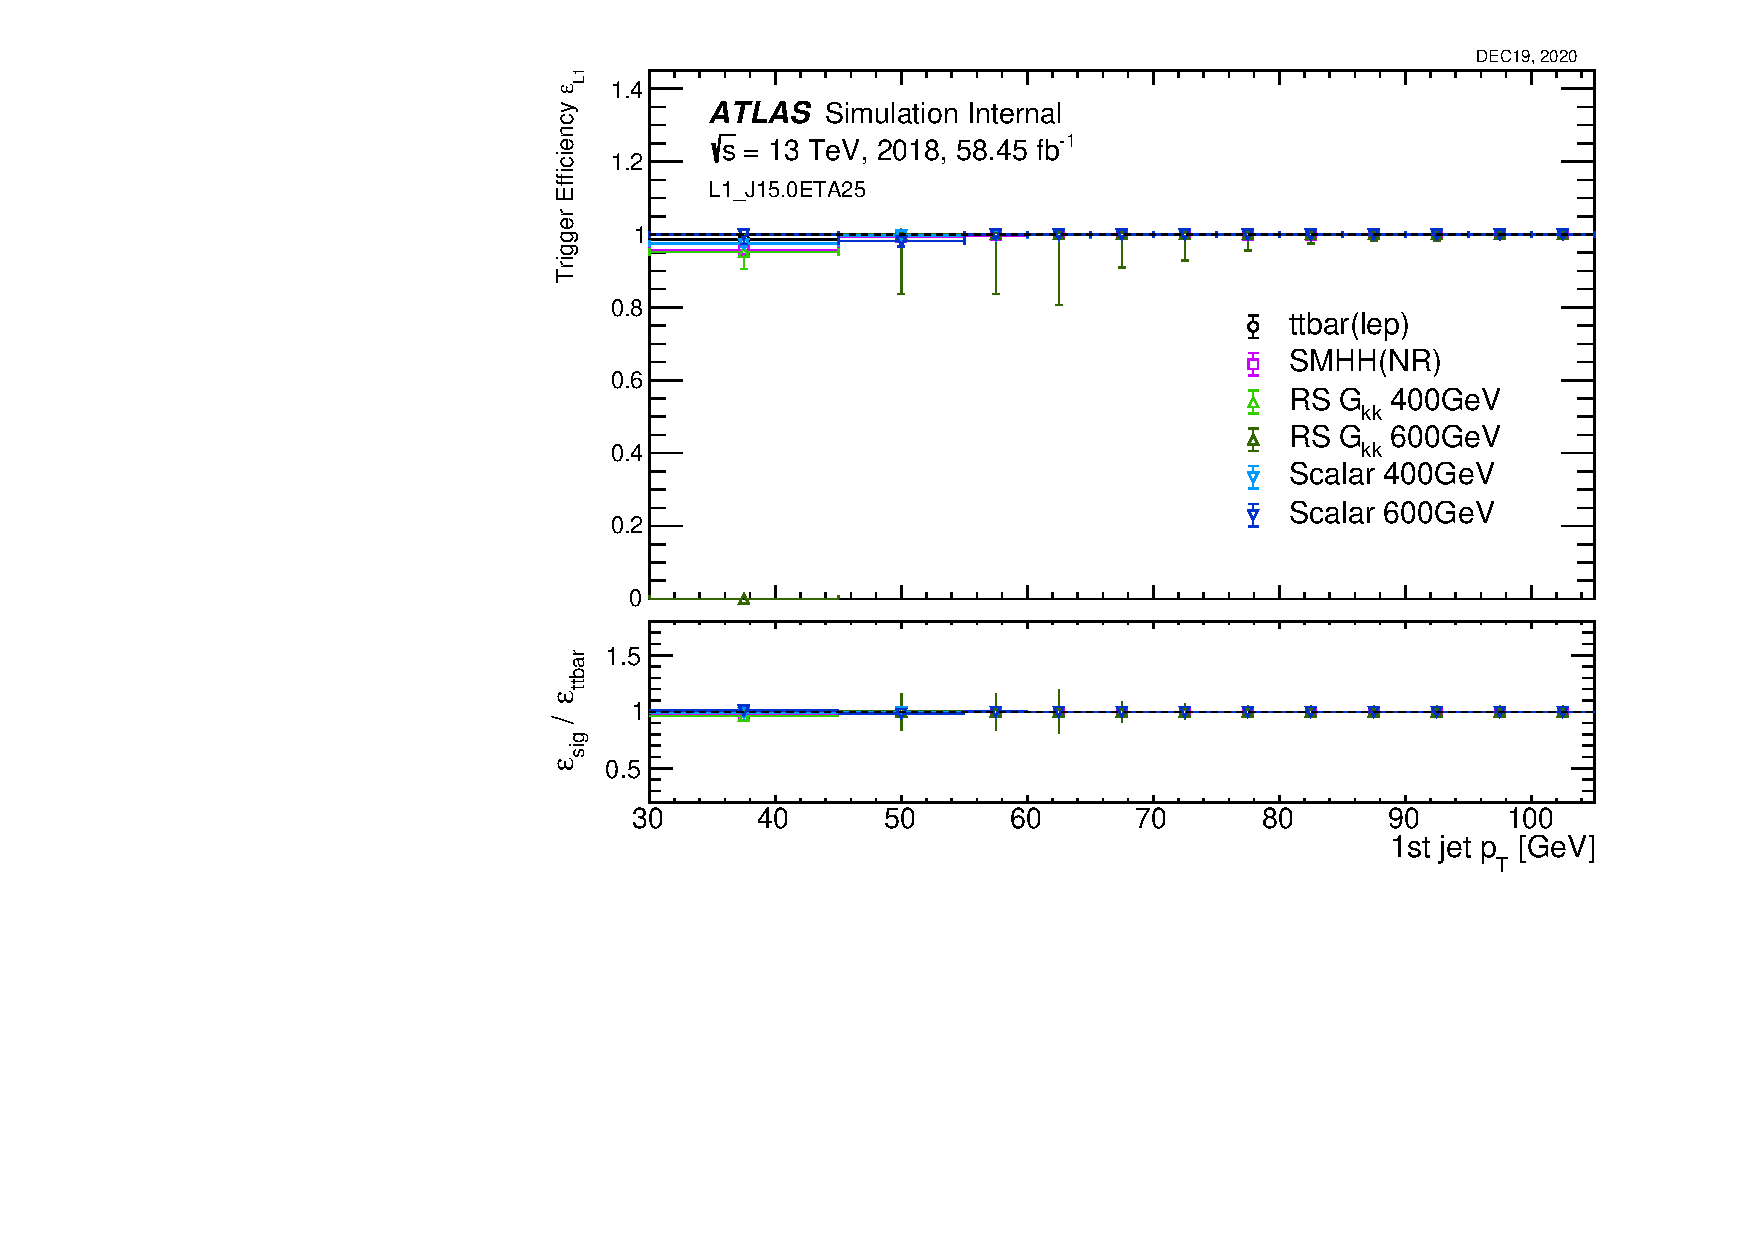
\includegraphics[width=0.25\textwidth]{\figpath{L1SDS/2018/sigDiff18-2b2j-L1-1st.pdf}}
    }   
    \subfloat[2nd jet at L1]{\label{fig:sigDiff18-2b2j-L1-2nd}%
            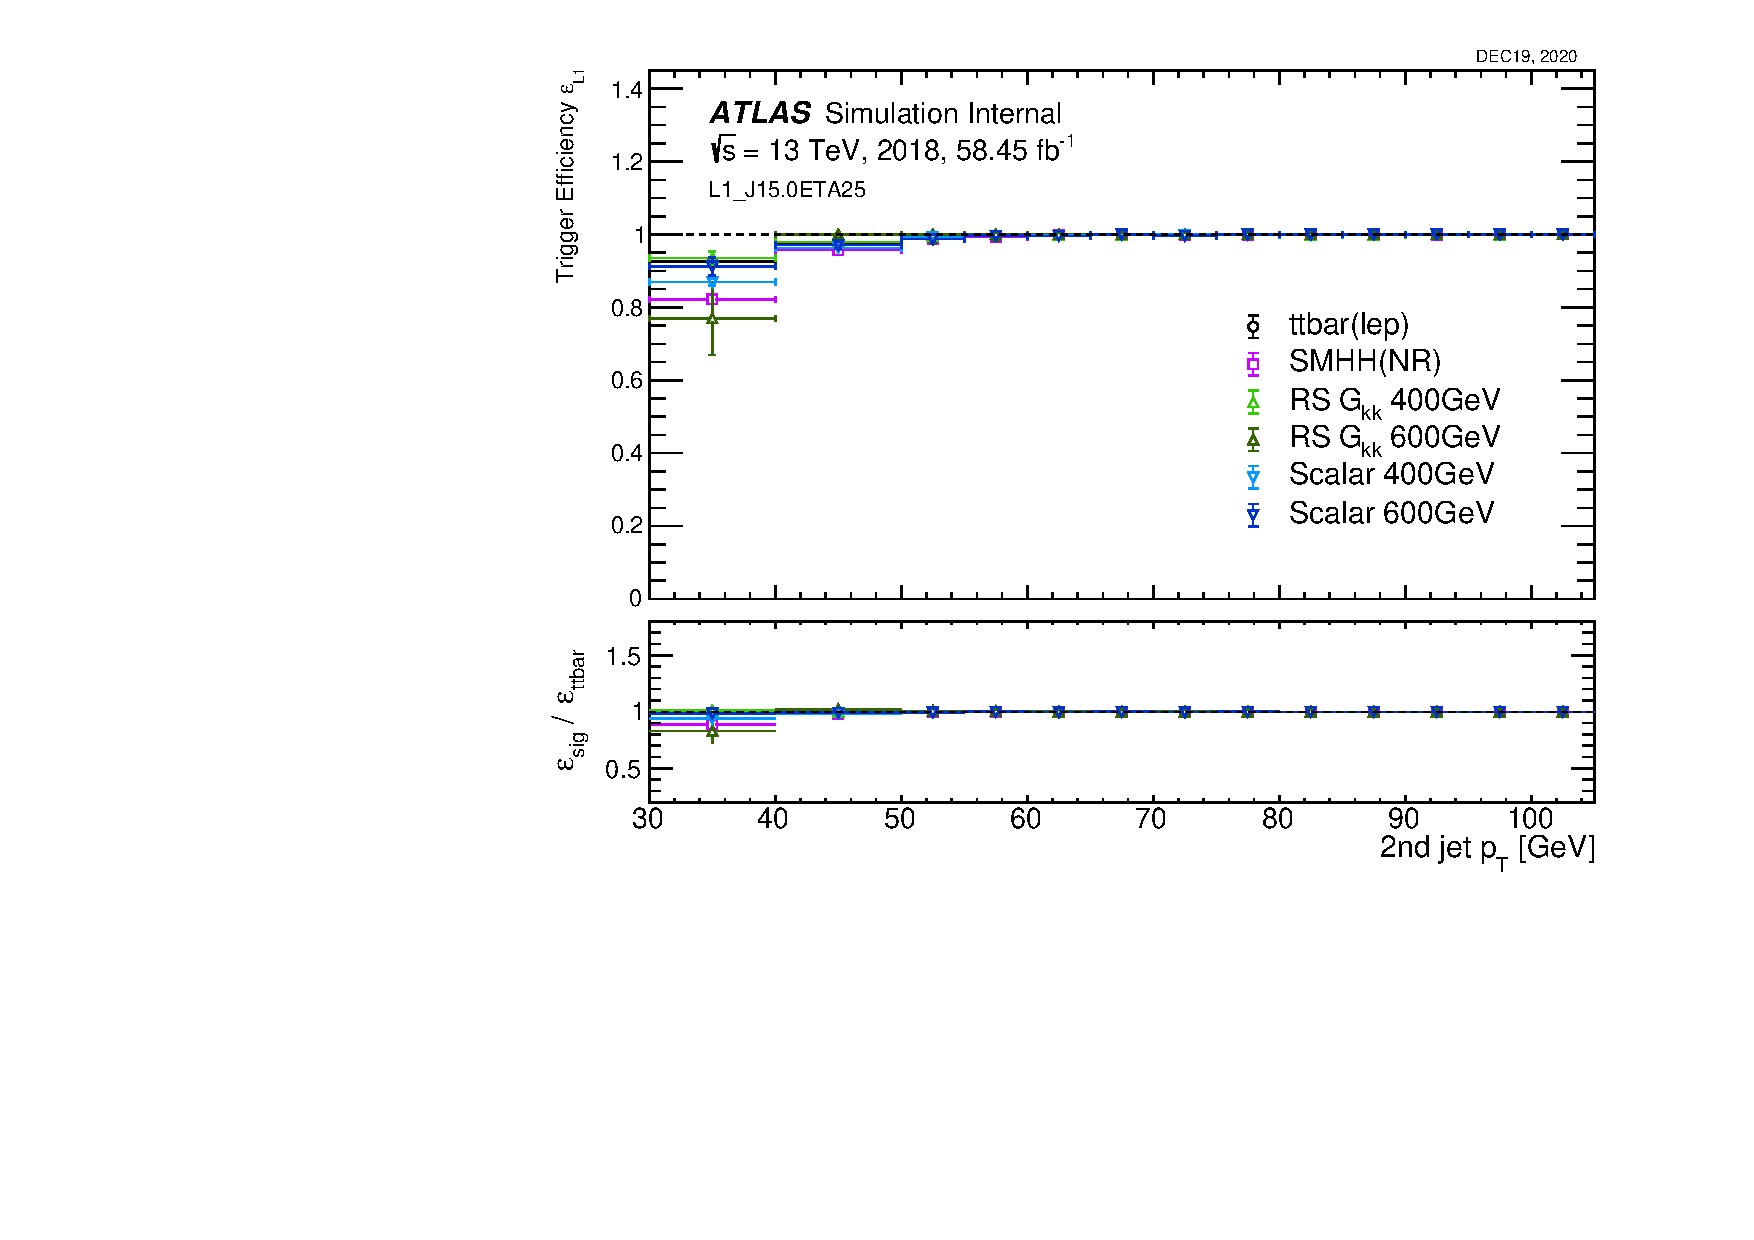
\includegraphics[width=0.25\textwidth]{\figpath{L1SDS/2018/sigDiff18-2b2j-L1-2nd.pdf}}
    }   
    \subfloat[3rd jet at L1]{\label{fig:sigDiff18-2b2j-L1-3rd}%
            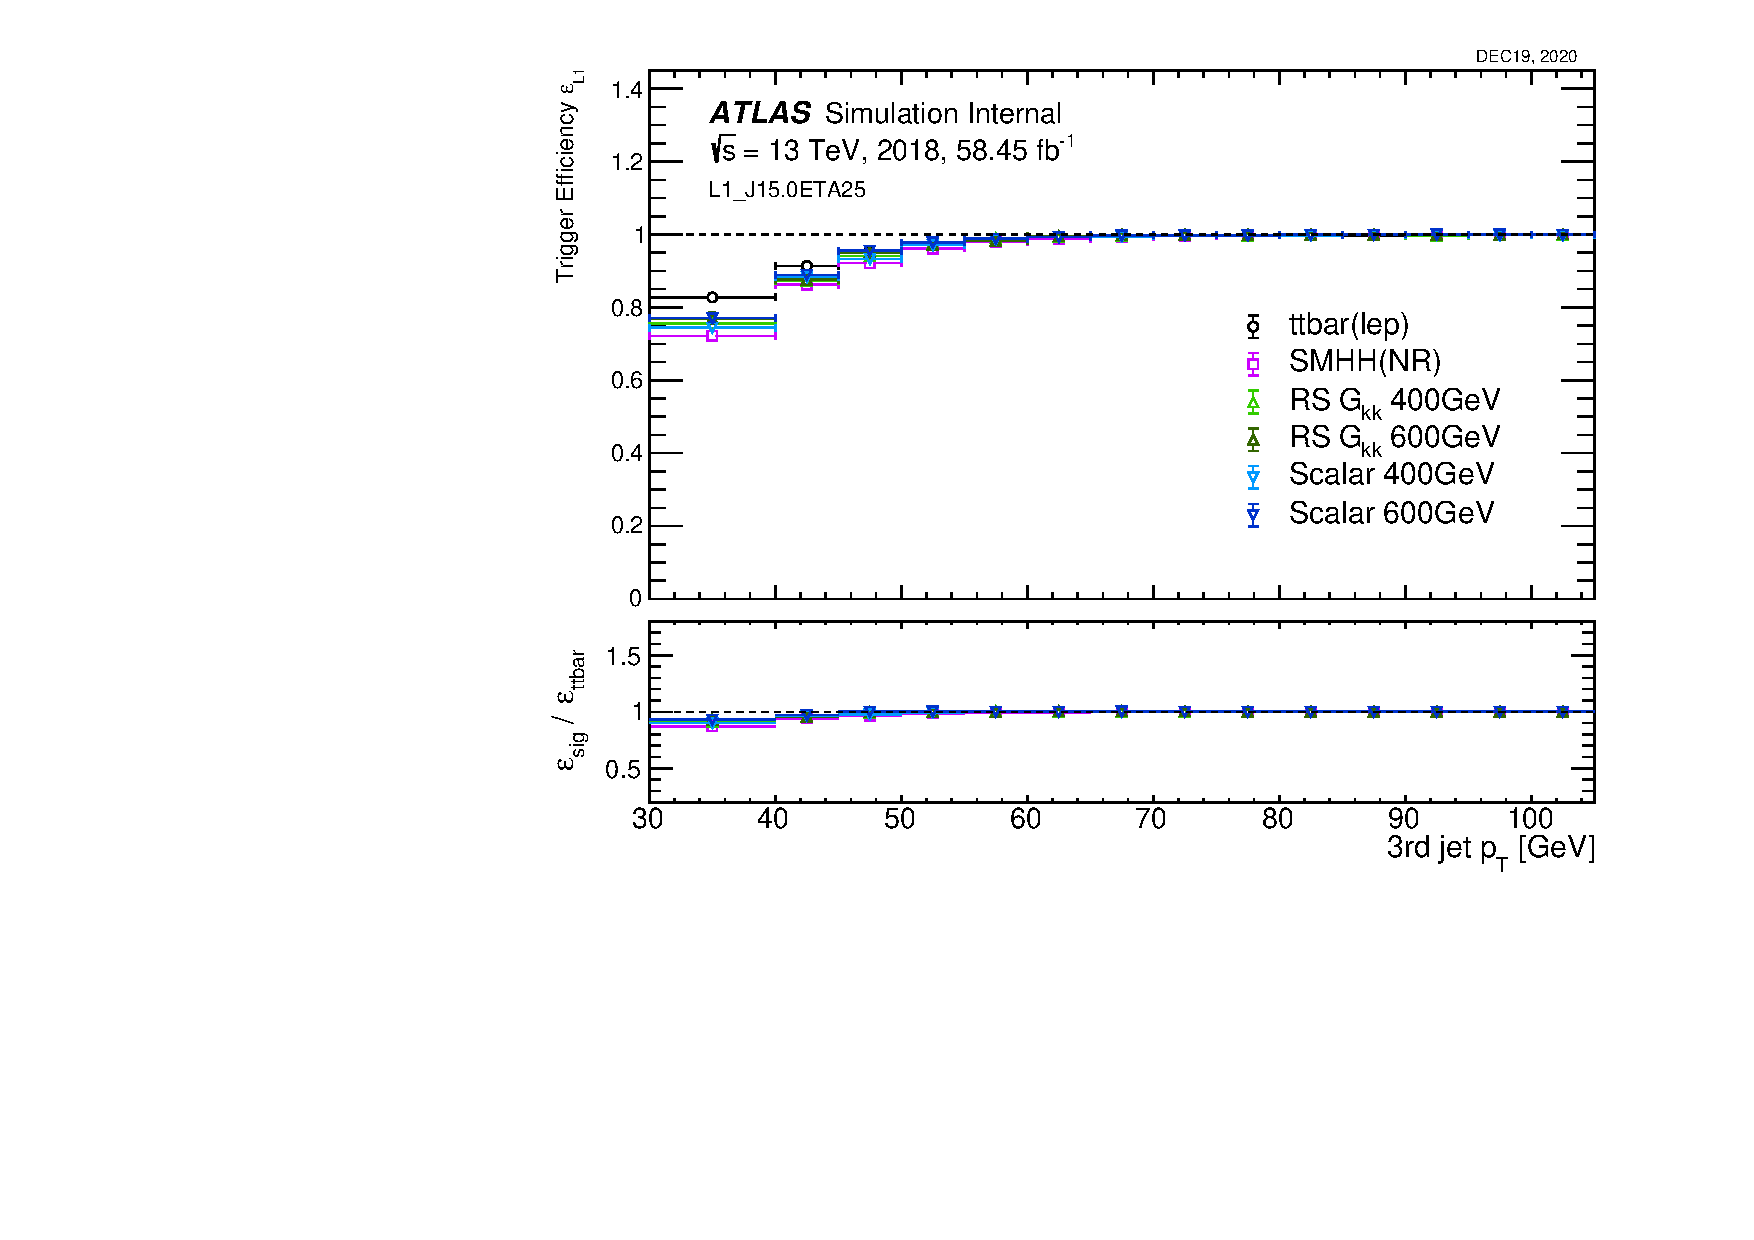
\includegraphics[width=0.25\textwidth]{\figpath{L1SDS/2018/sigDiff18-2b2j-L1-3rd.pdf}}
    }   
    \subfloat[4th jet at L1]{\label{fig:sigDiff18-2b2j-L1-4th}%
            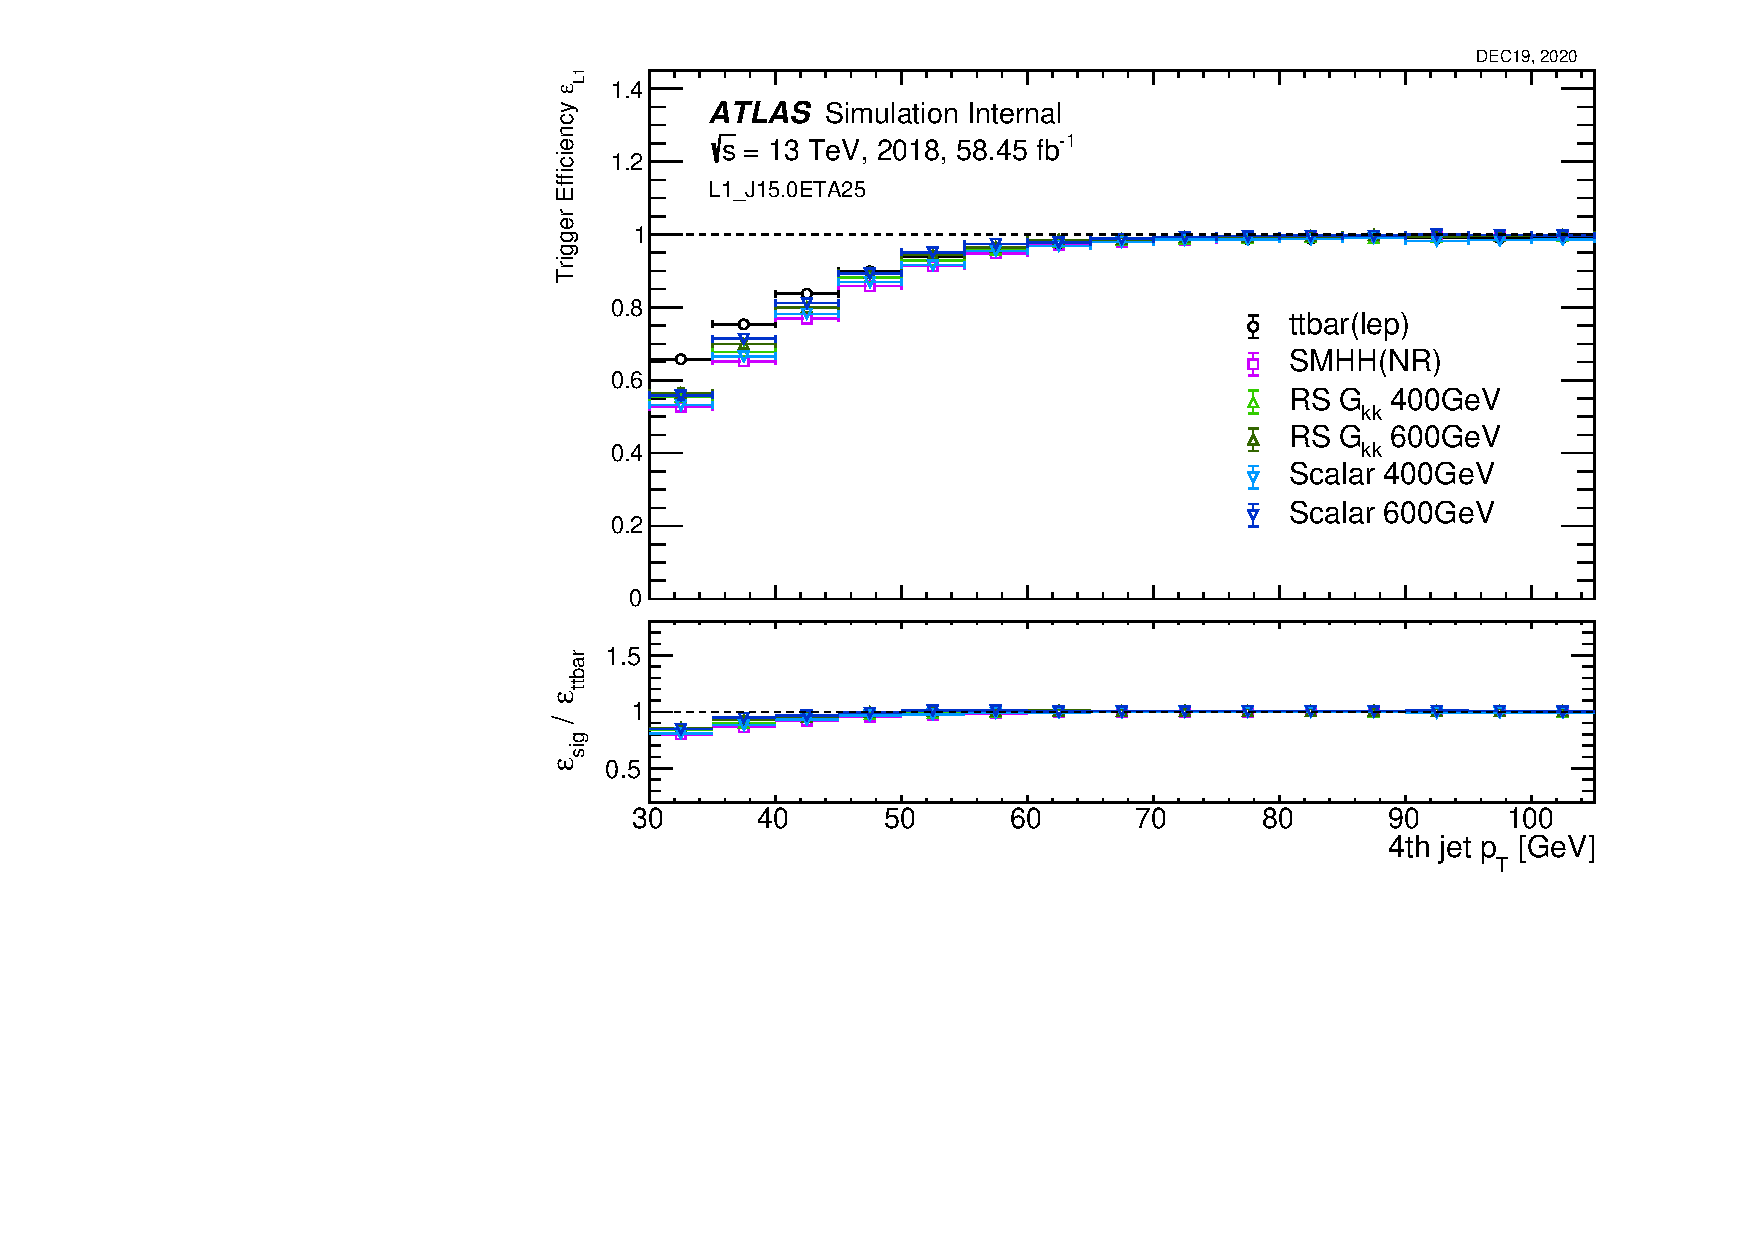
\includegraphics[width=0.25\textwidth]{\figpath{L1SDS/2018/sigDiff18-2b2j-L1-4th.pdf}}
    }   
 
    \subfloat[1st jet at HLT]{\label{fig:sigDiff18-2b2j-HLT-1st}%
            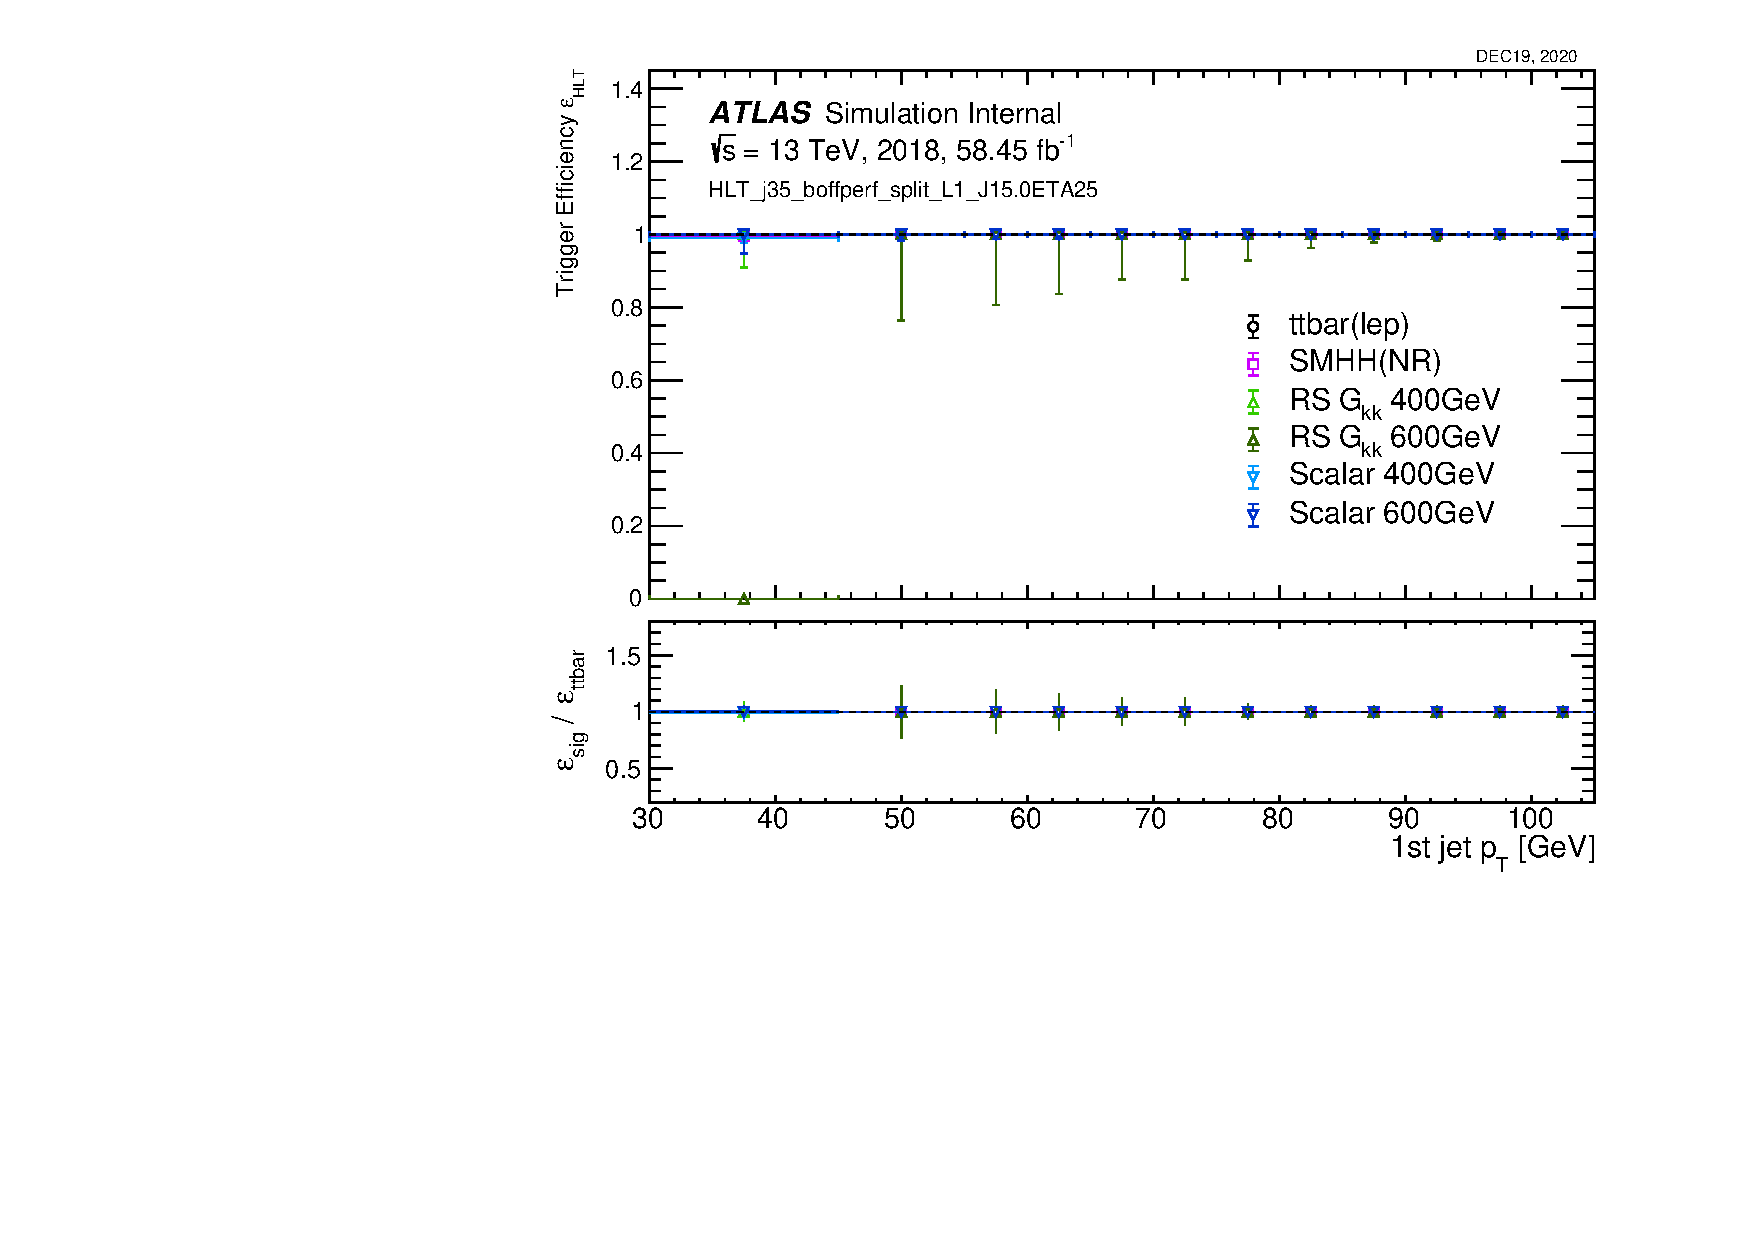
\includegraphics[width=0.25\textwidth]{\figpath{HLTSDS/2018/sigDiff18-2b2j-HLT-1st.pdf}}
    }   
    \subfloat[2nd jet at HLT]{\label{fig:sigDiff18-2b2j-HLT-2nd}%
            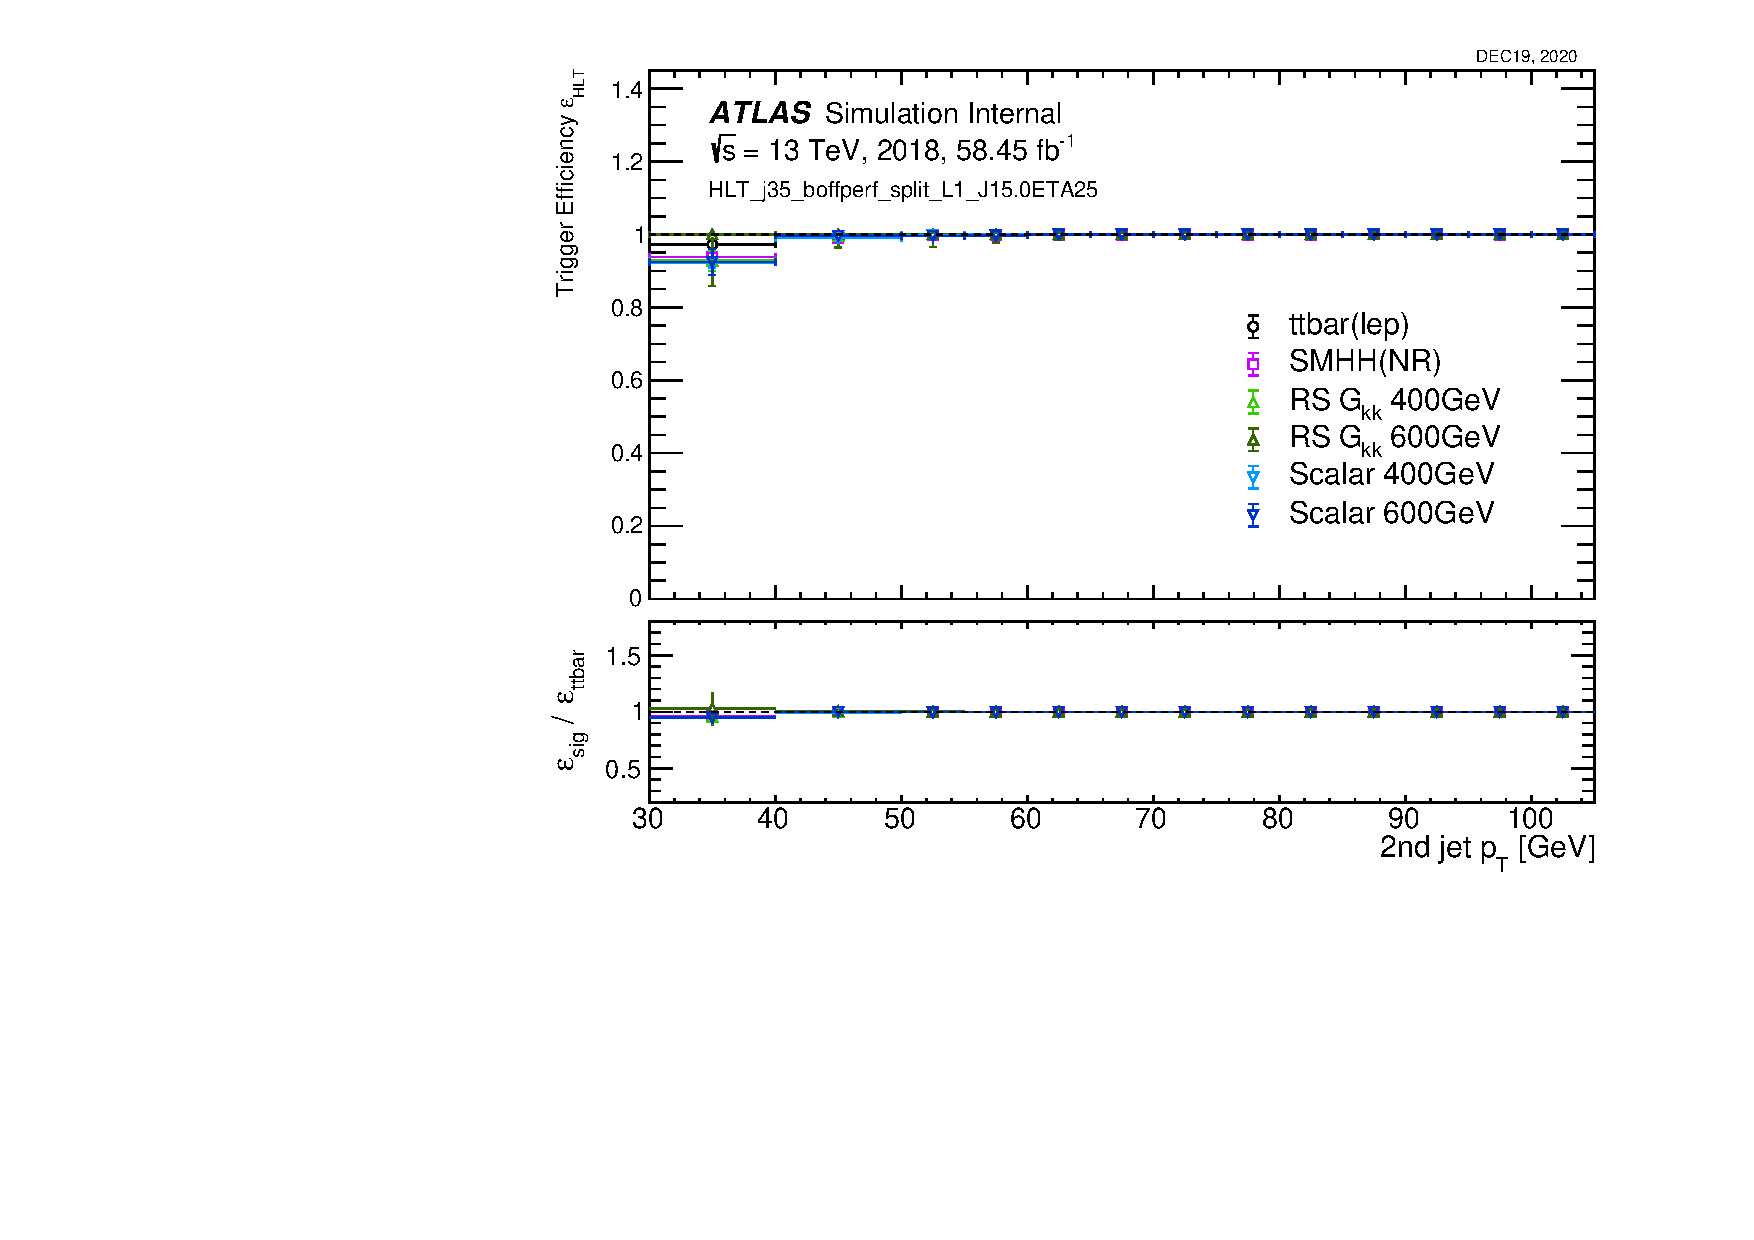
\includegraphics[width=0.25\textwidth]{\figpath{HLTSDS/2018/sigDiff18-2b2j-HLT-2nd.pdf}}
    }   
    \subfloat[3rd jet at HLT]{\label{fig:sigDiff18-2b2j-HLT-3rd}%
            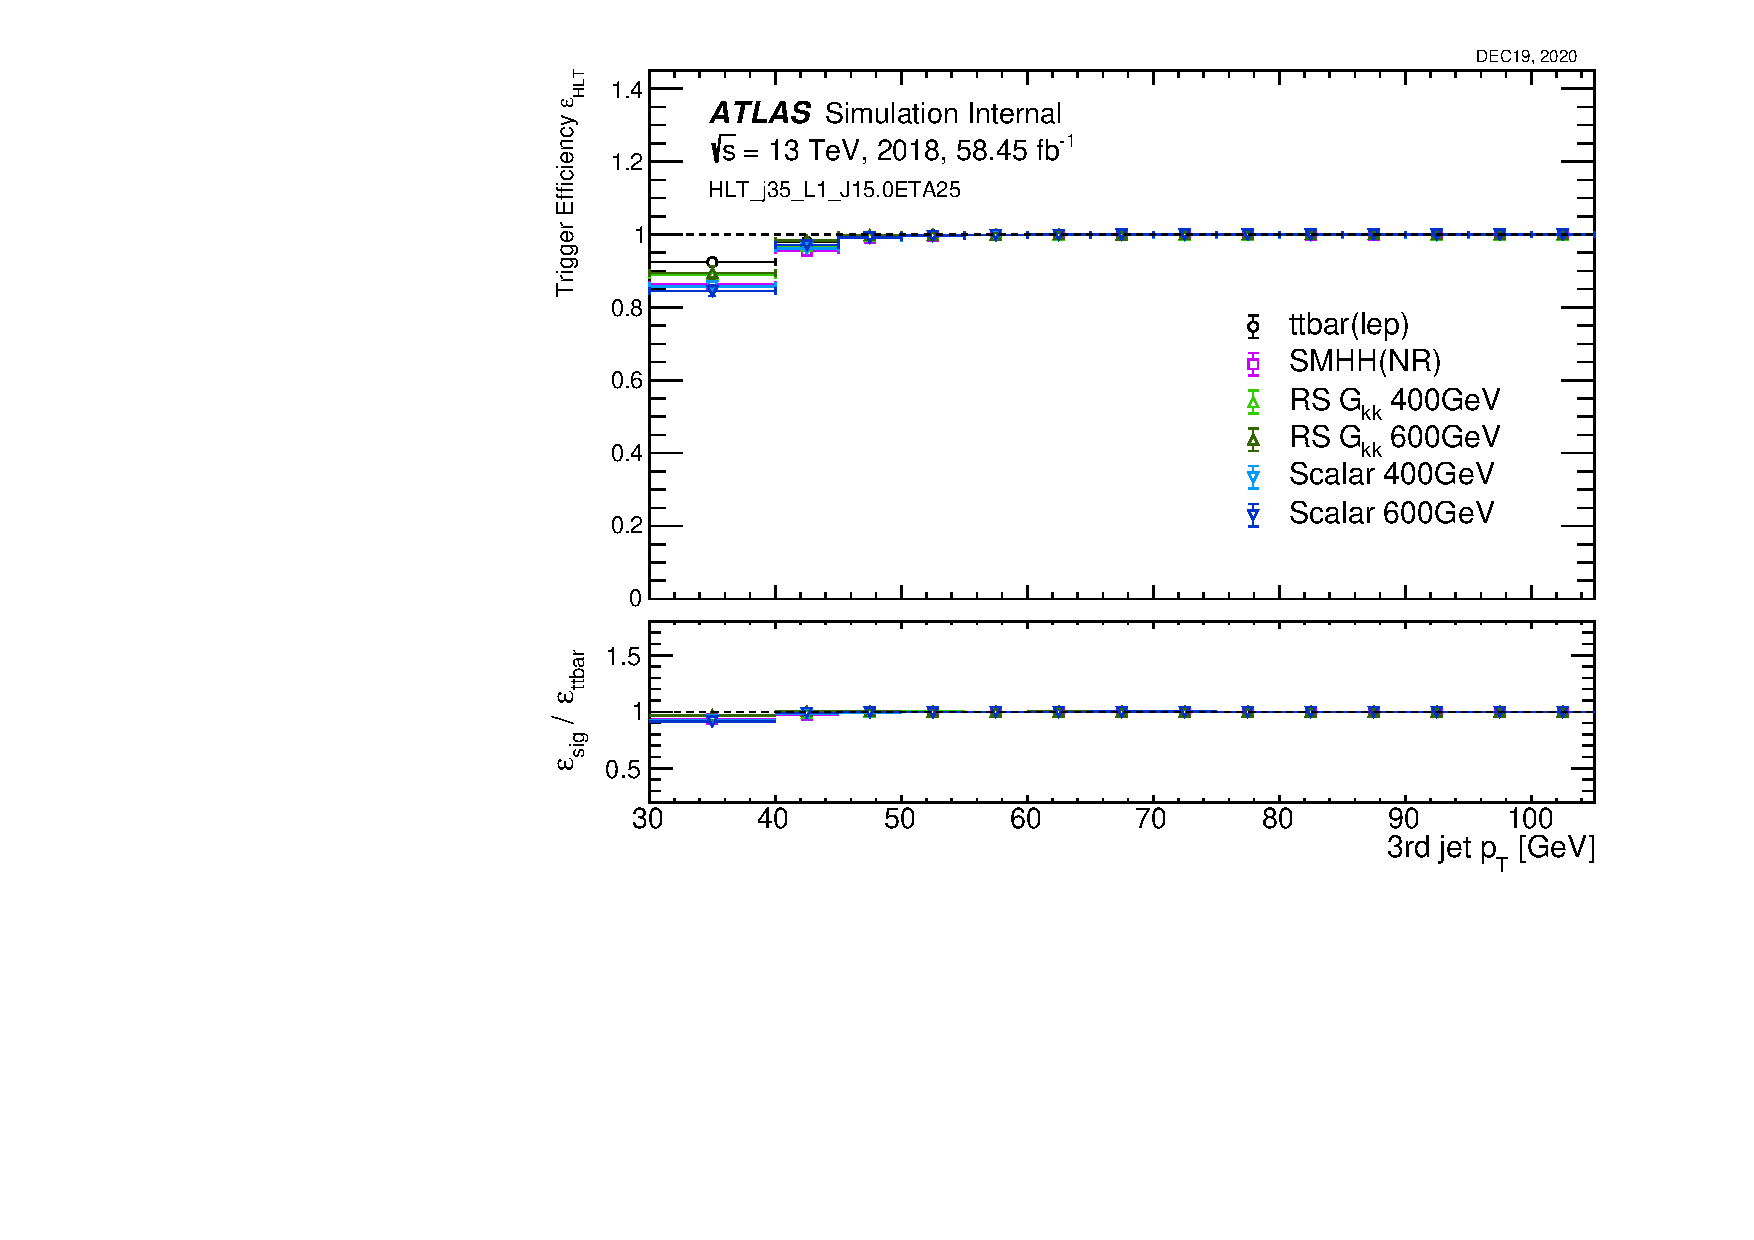
\includegraphics[width=0.25\textwidth]{\figpath{HLTSDS/2018/sigDiff18-2b2j-HLT-3rd.pdf}}
    }   
    \subfloat[4th jet at HLT]{\label{fig:sigDiff18-2b2j-HLT-4th}%
            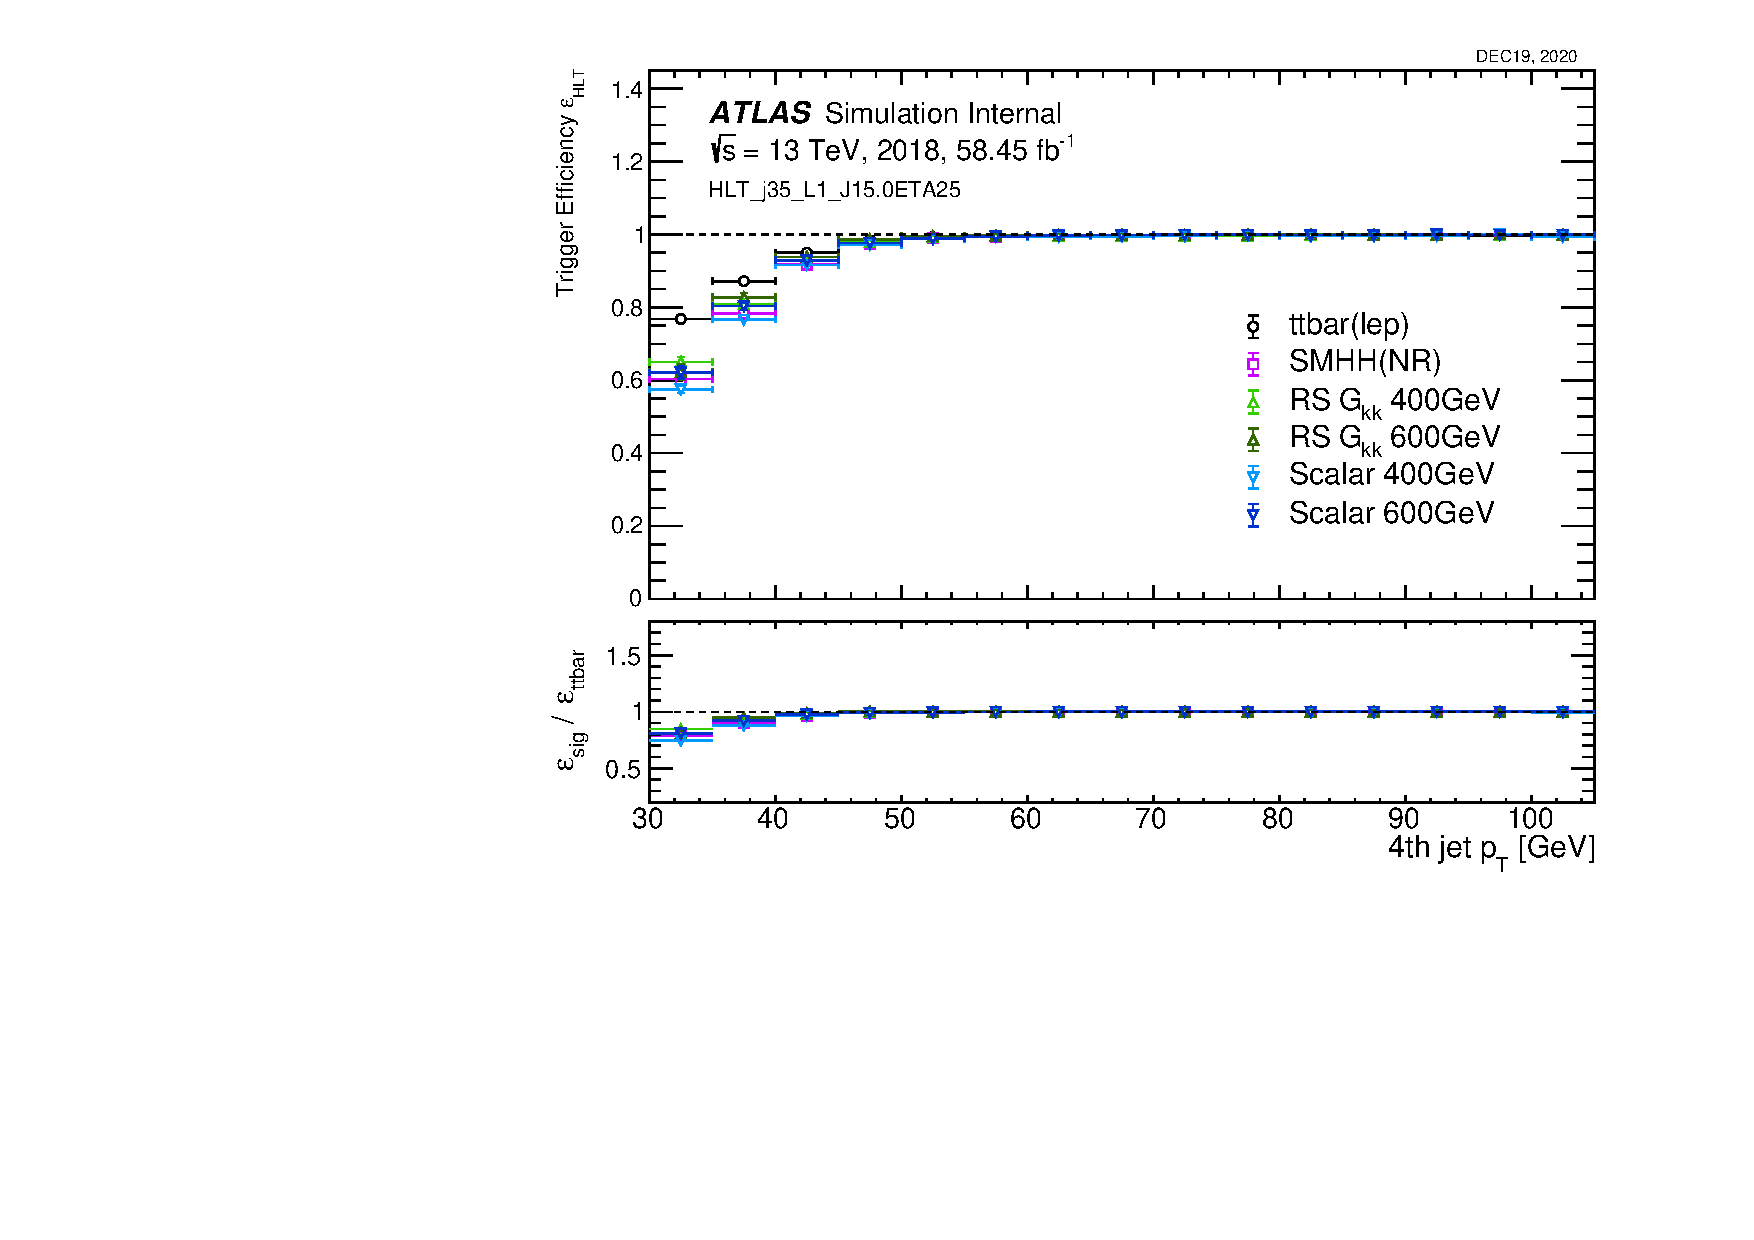
\includegraphics[width=0.25\textwidth]{\figpath{HLTSDS/2018/sigDiff18-2b2j-HLT-4th.pdf}}
    }   
    \caption{Jet-level trigger efficiencies of di-Higgs signals and semi-leptonic \ttbar in 2018 2b2j trigger as a function of offline jet \pt.
             The Nth jet is ordered by online \et.}
    \label{fig:sigDiff18-2b2j}
\end{figure}

